\documentclass[aspectratio=1610, professionalfonts, 13pt]{beamer}

% Lade das TU Dortund Theme von Max Nöthe
\usefonttheme[onlymath]{serif}
\usetheme[showtotalframes]{tudo}

% Lade richtiges Sprachpaket
\ifluatex
    \usepackage{polyglossia}
    \setmainlanguage{english}
\else
    \ifxetex
        \usepackage{polyglossia}
        \setmainlanguage{german}
    \else
        \usepackage[german]{babel}
    \fi
\fi

% Lade wichtige Mathematikpakete
\usepackage{amsmath}
\usepackage{amssymb}
\usepackage{mathtools}
\usepackage{cancel}
\usepackage[
  locale=DE,                   % deutsche Einstellungen
  separate-uncertainty=true,   % Immer Fehler mit \pm
  per-mode=symbol-or-fraction, % m/s im Text, sonst Brüche
]{siunitx}
\usepackage[absolute,overlay]{textpos}
\usepackage{framed}
\usepackage{multicol}
\usepackage{setspace}
\usepackage{graphicx}
\usepackage{booktabs}
\usepackage{caption}
\usepackage{appendixnumberbeamer}
\usepackage{tikz}
\usepackage[export]{adjustbox}
\usepackage{color}


% Lade Paket zur Nutzung von Schleifen
\usepackage{forloop}

% ------------------------- Präsentationsinformationen -------------------------

% Titel:
\title{\textbf{Tracker calibration studies in FairShip}}
\subtitle{SHiP}

% Autoren:
\author{Kevin Sedlaczek}

% Datum:
\date{July to September 2017}

% Lehrstuhl/Fakultät:
\institute[CERN]{Summer Student Programme}

% Titelgrafik:
\titlegraphic{
\includegraphics[width=0.2\textwidth]{logos/CERN-logo.jpg}\hfill
\includegraphics[width=0.2\textwidth]{logos/SHiP-Full_Black_0.png}}

% ------------------------------------------------------------------------------


\begin{document}

\maketitle

%-------------------------------INHALT EINFÜGEN---------------------------------

\begin{frame}[t]{content}
  \begin{enumerate} \setlength\itemsep{0.5cm}
    \item {\Large motivation}
    \item {\Large data sets}
    \item {\Large reconstructed distance to target}
    \item {\Large particle flux in strawtubes}
    \item {\Large summary}
    \item {\Large outlook}
  \end{enumerate}
\end{frame}

%------------------------------------------------------------------------------------------
\section{motivation}
%------------------------------------------------------------------------------------------

\begin{frame}[t]{motivation}
  \begin{multicols}{2}
    \begin{figure}
      \centering
      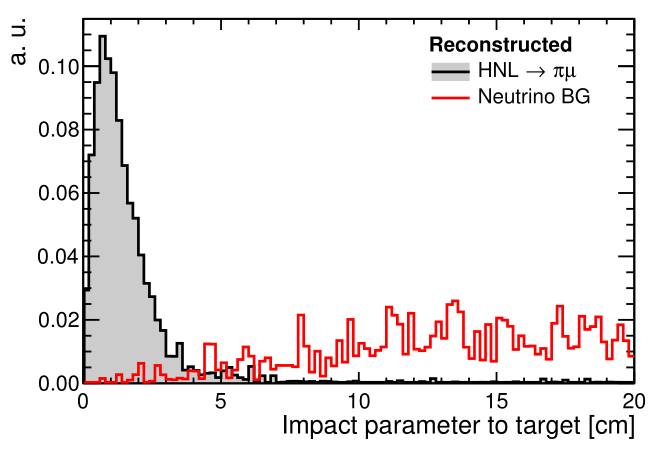
\includegraphics[width=0.5\textwidth]{IP_cut.png}
    \end{figure}
    \columnbreak
    \vspace*{\fill}
      \begin{enumerate}
        \item check for reconstruction effects on MC truth
        \item reconstruct target position from measured tracks?
        \item cuts on IP for analysis
        \item calibration of strawtubes
        \item $\rightarrow$ what is the expected flux at tracker?
      \end{enumerate}
    \vspace*{\fill}
  \end{multicols}
\end{frame}

%------------------------------------------------------------------------------------------
\section{data sets}
%------------------------------------------------------------------------------------------
\begin{frame}[t]{Used data sets}
  \begin{itemize}
    \item Working with different samples that vary in the \textbf{magnetic field of the muon shield}
    \item Constructed via the FairShip framework
    \begin{itemize}
      \item \texttt{run\_SimScript.py} with flags \texttt{--MuonBack --FollowMuon} and \texttt{--Field} customized to change the field of the muon shield.
      \item \texttt{ShipReco.py} to simulate the reconstruction and detector
      \item files with different magnetic fields \texttt{muShield.B} of the muon shield
      \item And also without any magnetic field in all detector components before T1 (\texttt{c.tauMS.B}$=\SI{1.5}{\tesla}$/\texttt{c.EmuMagnet.B}$=\SI{1}{\tesla}$)
      \item samples with 100\,000 events
    \end{itemize}
  \end{itemize}
\end{frame}

%------------------------------------------------------------------------------------------
\section{Target IP}
%------------------------------------------------------------------------------------------


%\begin{frame}[t]{reconstructed distances to the target}
%  \begin{itemize}
%    \item possible to use reconstructed coordinates at target as a selection criterium?
%    \item real production vertex in MC truth
%    \item reconstructed tracks offer momenta of particles at certain points in the detector
%    \item one can use this information to linearly extrapolate back to the target z-postion
%  \end{itemize}
%\end{frame}

\begin{frame}[t]
  \vspace*{\fill}
    \centering
    {\huge Calculated distance to target (impact parameter)}
  \vspace*{\fill}
\end{frame}


\begin{frame}[t]{Calculation of impact parameter}
    The reconstructed tracks (namely the fitted states) are accessed via:
    \begin{figure}
      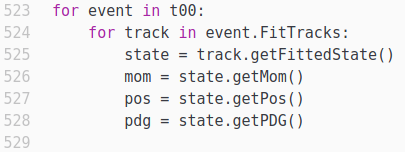
\includegraphics[width=0.4\textwidth,left]{loop.png}
    \end{figure}
    They yield a spatial vector $\vec{r}_\text{track}=(x,y,z)$ and a momentum vector $\vec{p}=(p_x,p_y,p_z)$. The spatial vector is used as a starting point, while the momentum vector defines the direction. The so defined straight line in 3D space can then be extrapolated to the z-component of the target centre.
\end{frame}

\begin{frame}[t]{}
  \begin{figure}
    \centering
    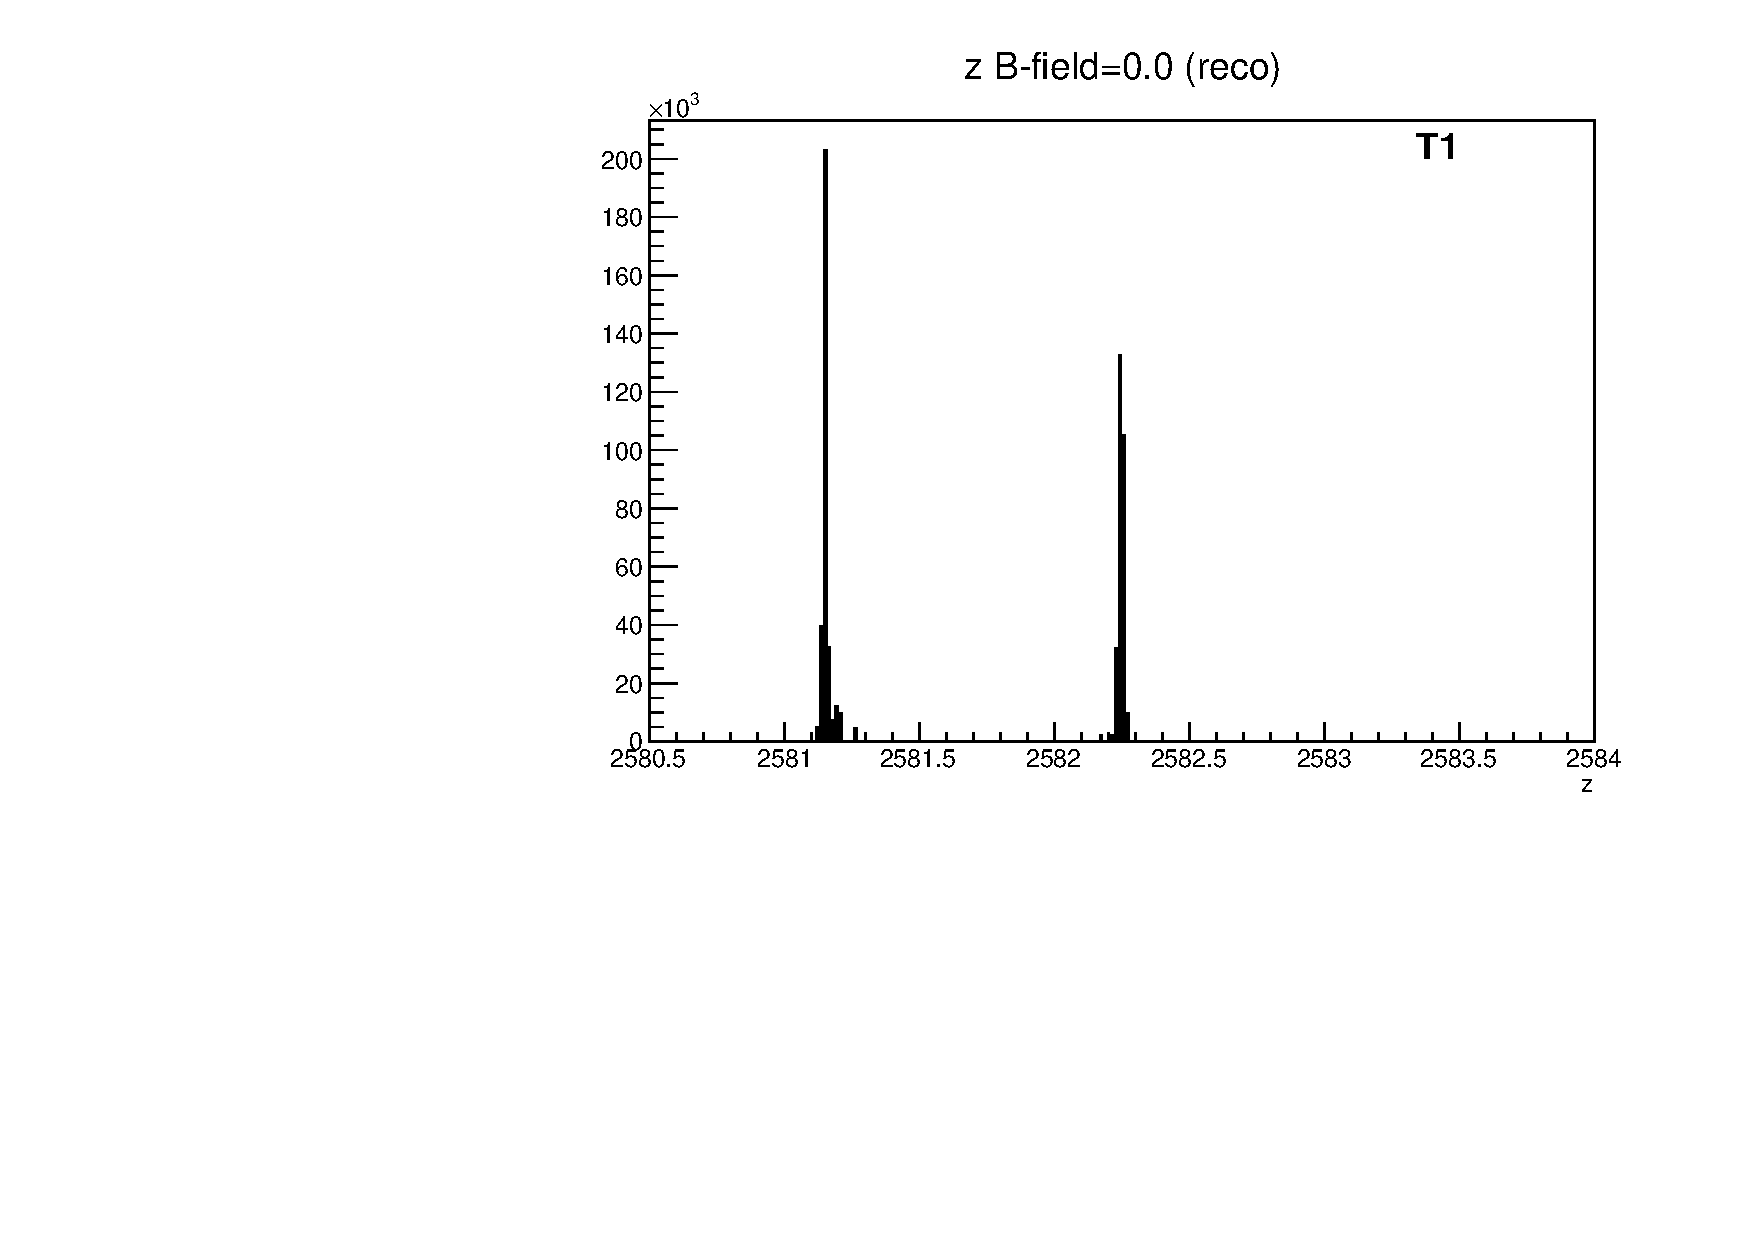
\includegraphics[width=0.65\textwidth]{../hists/nofield/z_1M.pdf}
  \end{figure}
\end{frame}

\begin{frame}[t]{Calculation of impact parameter}
  \begin{itemize}
    \item The target centre is located at $z_t=-7067.0$, so that the $x$ and $y$ coordinates of the fitted tracks can be calculated.
    \item So the track is described by
  \end{itemize}
  %
  \begin{equation}
    \vec{r}(t)=\vec{p}\cdot t+\vec{r}_\text{track}
  \end{equation}
  Thus one only needs to calculate the $t$ for the $z$-component and apply it to $x$ and $y$.
  \begin{itemize}
    \item $t = \frac{z_\text{target}-z}{p_z}$
    \item $x_\text{target} = p_x\cdot t + x$
    \item $y_\text{target} = p_y\cdot t + y$
    \item this then gives the distance in the $x$-$y$-plane: $d = \sqrt{x_\text{target}^2+y_\text{target}^2}$
  \end{itemize}
\end{frame}

\begin{frame}[t]{}
  \begin{figure}
    \centering
    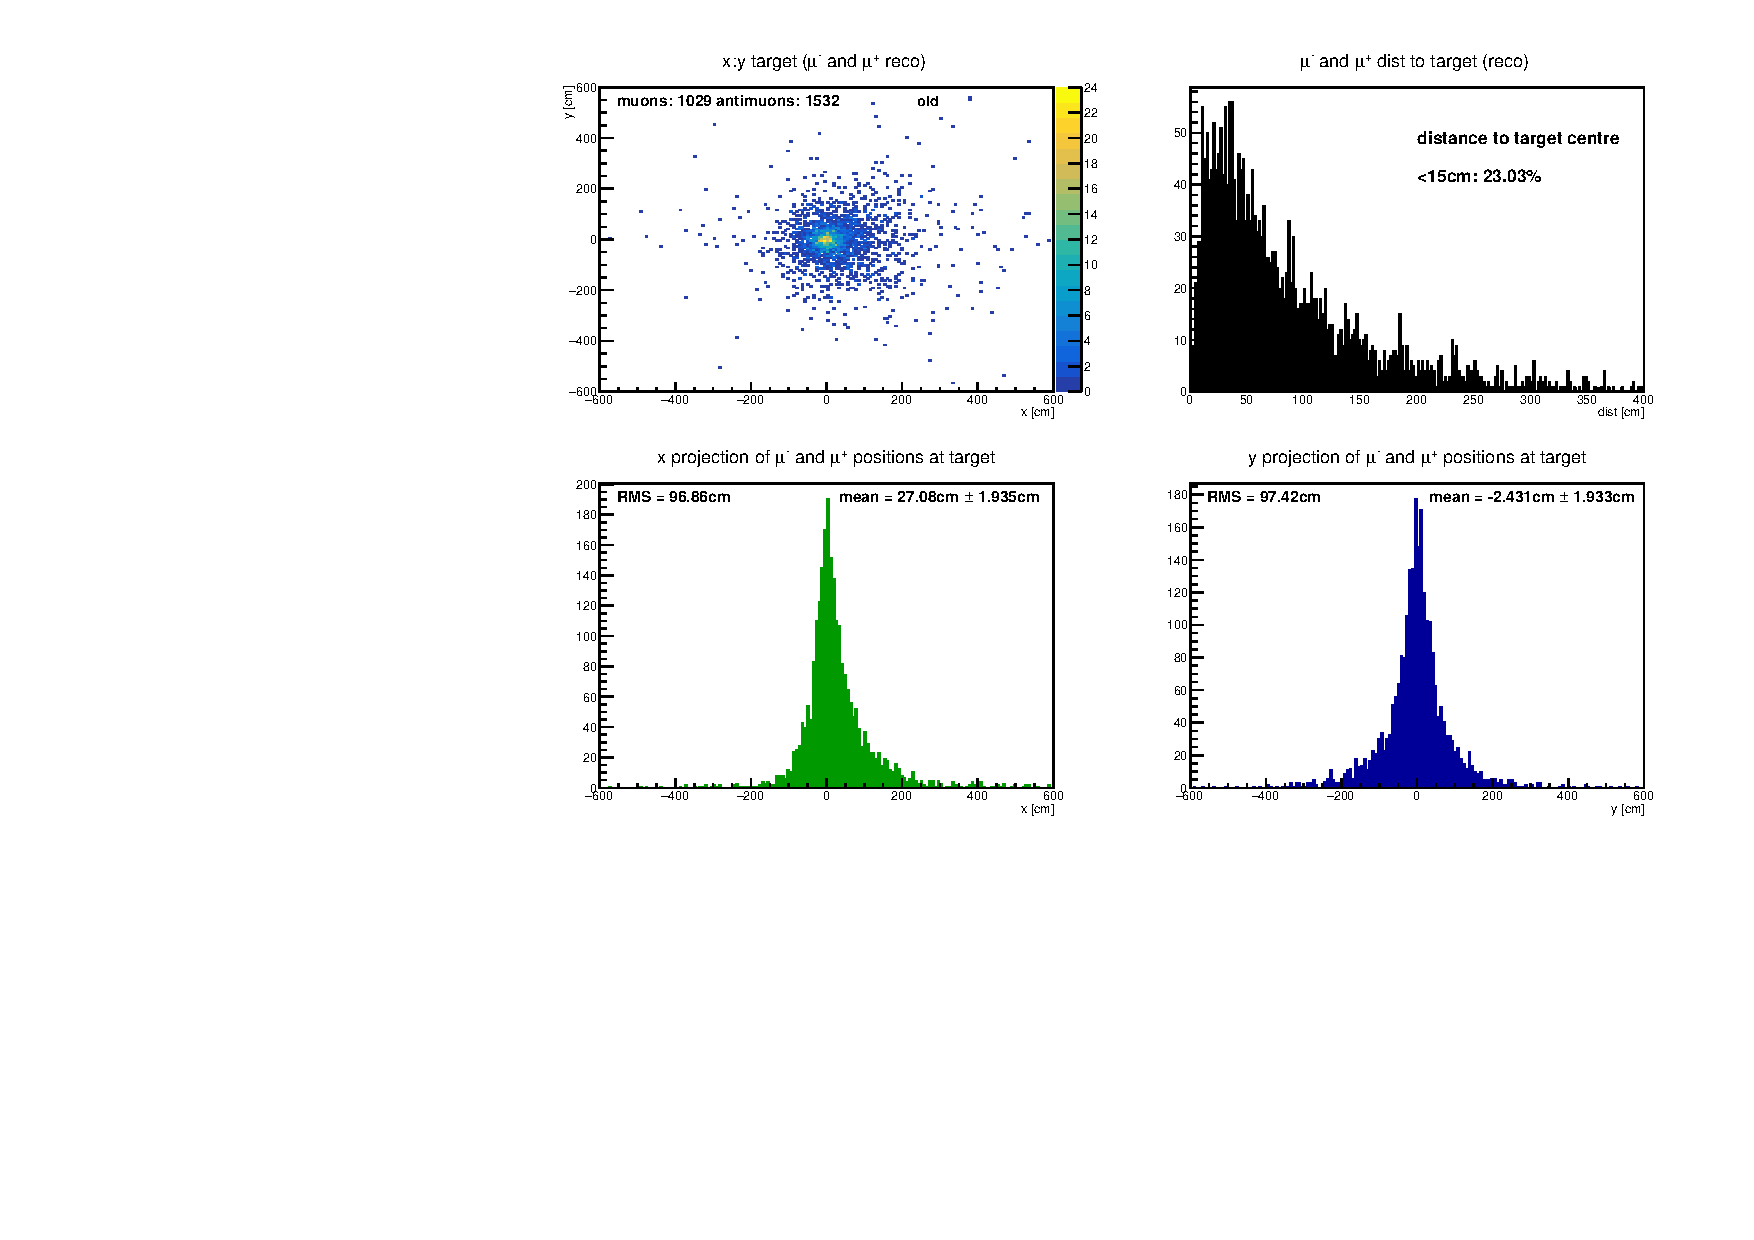
\includegraphics[width=0.75\textwidth]{../hists/nofield/old/target_dist.pdf}
  \end{figure}
\end{frame}


\begin{frame}
  \begin{table}
    \centering
    \begin{tabular}{c
                    S
                    S
                    S}
      \toprule
      {$\mu^{+}$} & {all momenta} & {$p>\SI{10}{\giga\electronvolt}$} & {$p<\SI{10}{\giga\electronvolt}$} \\
      \midrule
      mean $x$ /cm & 23.84(238) & 9.4(15) & 53.37(639) \\
      mean $y$ /cm & -0.733(2356) & -0.12(156) & -1.93(626) \\
      RMS $x$ /cm & 92.28 & 46.73 & 142.1 \\
      RMS $y$ /cm & 92.27 & 49.6 & 142.7 \\
      \midrule
      {$\mu^{-}$} & {all momenta} & {$p>\SI{10}{\giga\electronvolt}$} & {$p<\SI{10}{\giga\electronvolt}$} \\
      \midrule
      mean $x$ /cm & 29.31(317) & 8.13(195) & 64.38(745)  \\
      mean $y$ /cm & 9.931(3128) & 1.725(1902) & 22.95(746)  \\
      RMS $x$ /cm & 102.3 & 49.74 & 147.4  \\
      RMS $y$ /cm & 102 & 48.58 & 151.3  \\
      \bottomrule
    \end{tabular}
    \caption{Means and RMS of the $x$- and $y$-projections of the reconstructed IP.}
    \label{tab:mean}
  \end{table}
\end{frame}

\begin{frame}[t]{Dependence of asymmetry}
  \begin{itemize}
    \item asymmetry in x-projection: mean shifted to one side
    \item mostly independent of charge of the muon
    \item momentum dependence: x- distribution moves to the same direction for both charges when setting momentum cuts
  \end{itemize}
\end{frame}

\begin{frame}[t]{}
  \begin{figure}
    \centering
    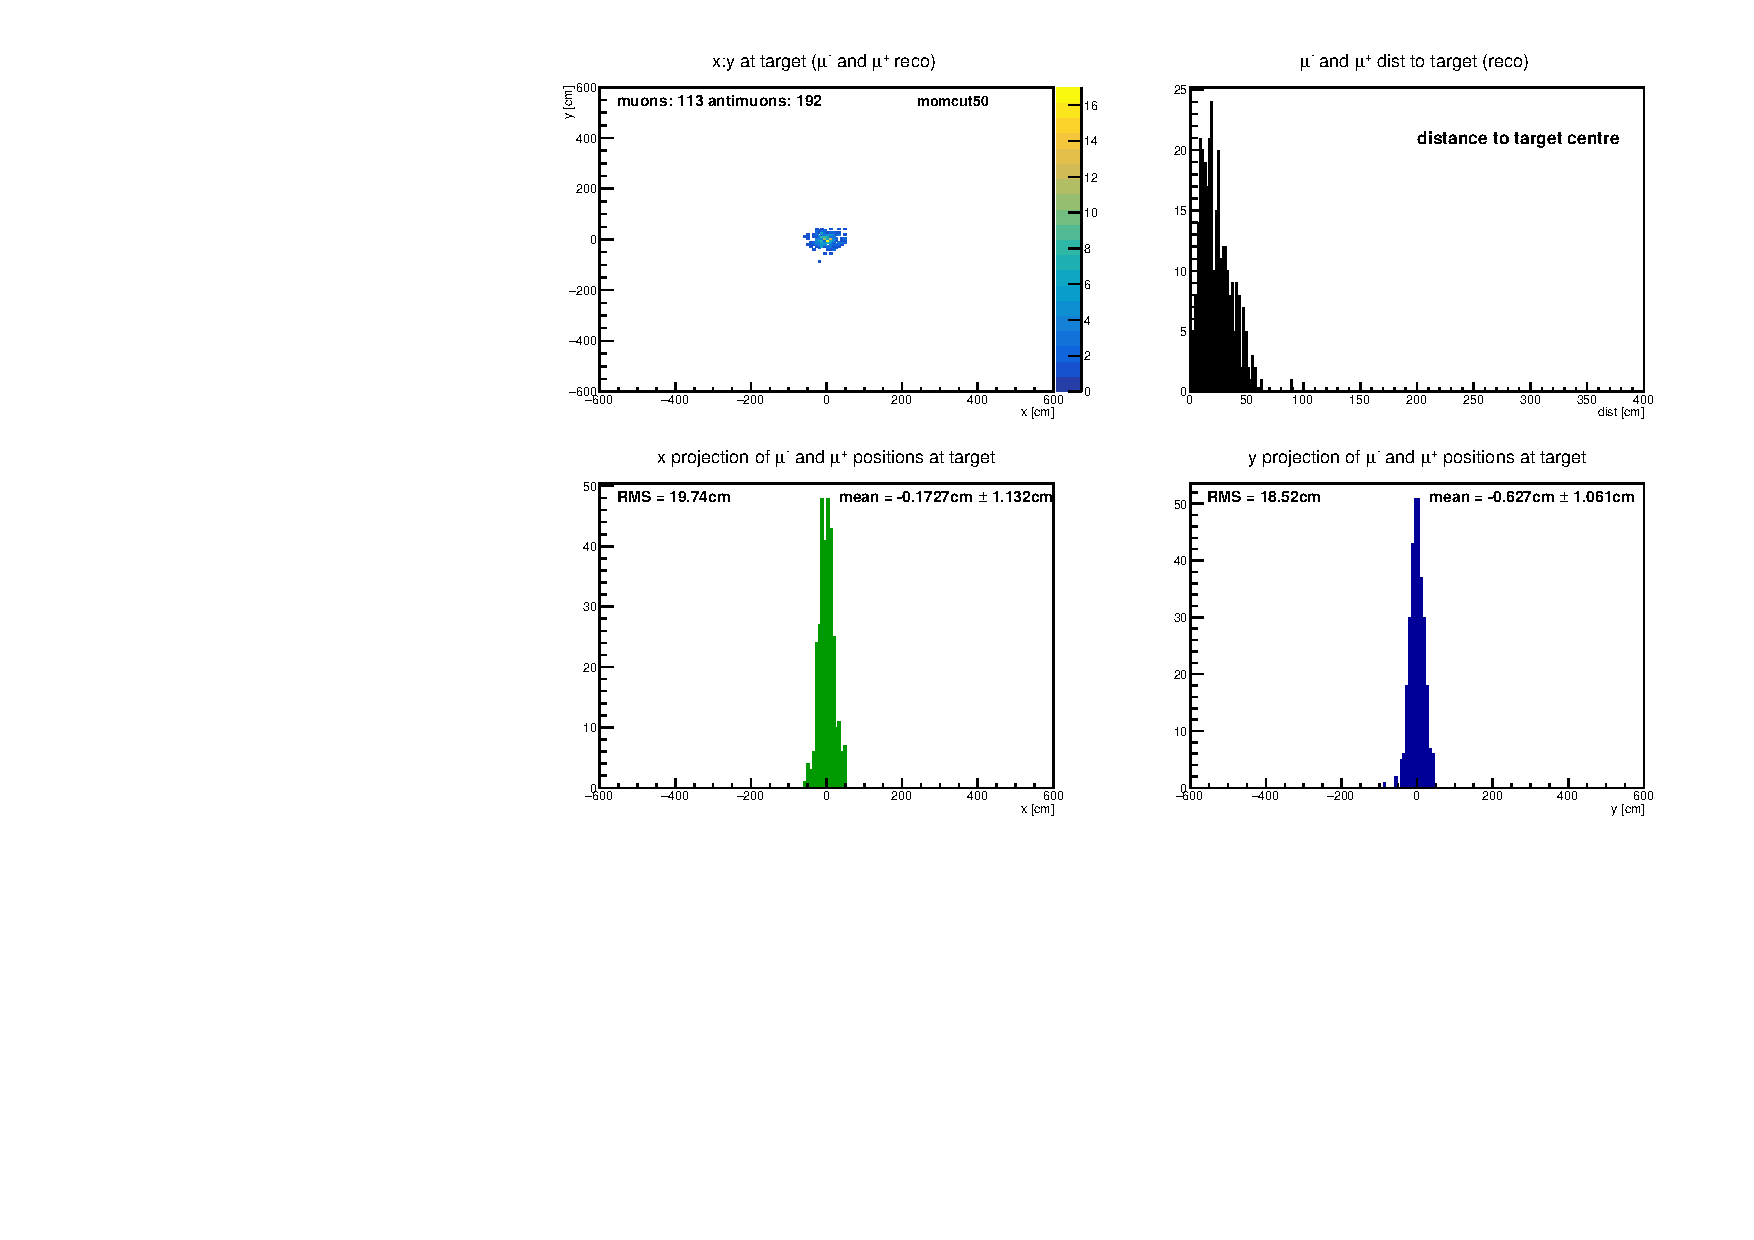
\includegraphics[width=0.65\textwidth]{../hists/nofield/momcut50/target_dist.pdf}
  \end{figure}
\end{frame}

\begin{frame}[t]{Dependence of asymmetry}
  \begin{itemize}
    \item asymmetry in x-projection: mean shifted to one side
    \item mostly independent of charge of the muon
    \item momentum dependence: x- distribution moves to the same direction for both charges when setting momentum cuts
    \item almost gone for momentum-cut above $\SI{50}{\giga\electronvolt}$
  \end{itemize}
  Also occured when using the extrapolator to go to $z=0$ and using a linear fit to go to the target. \\ Looking at the slopes of the true MC muon tracks, there were only muons with px>0 and py==0. \\
  \begin{framed}
    fix \textbf{bug} in MuonBackGenerator: phi=0 was used if phismearing was off instead of true phi
  \end{framed}
\end{frame}


%------------------------------------------------------------------------------------------
\section{old data samples}
%------------------------------------------------------------------------------------------

\begin{frame}[t]{}
  \begin{figure}
    \centering
    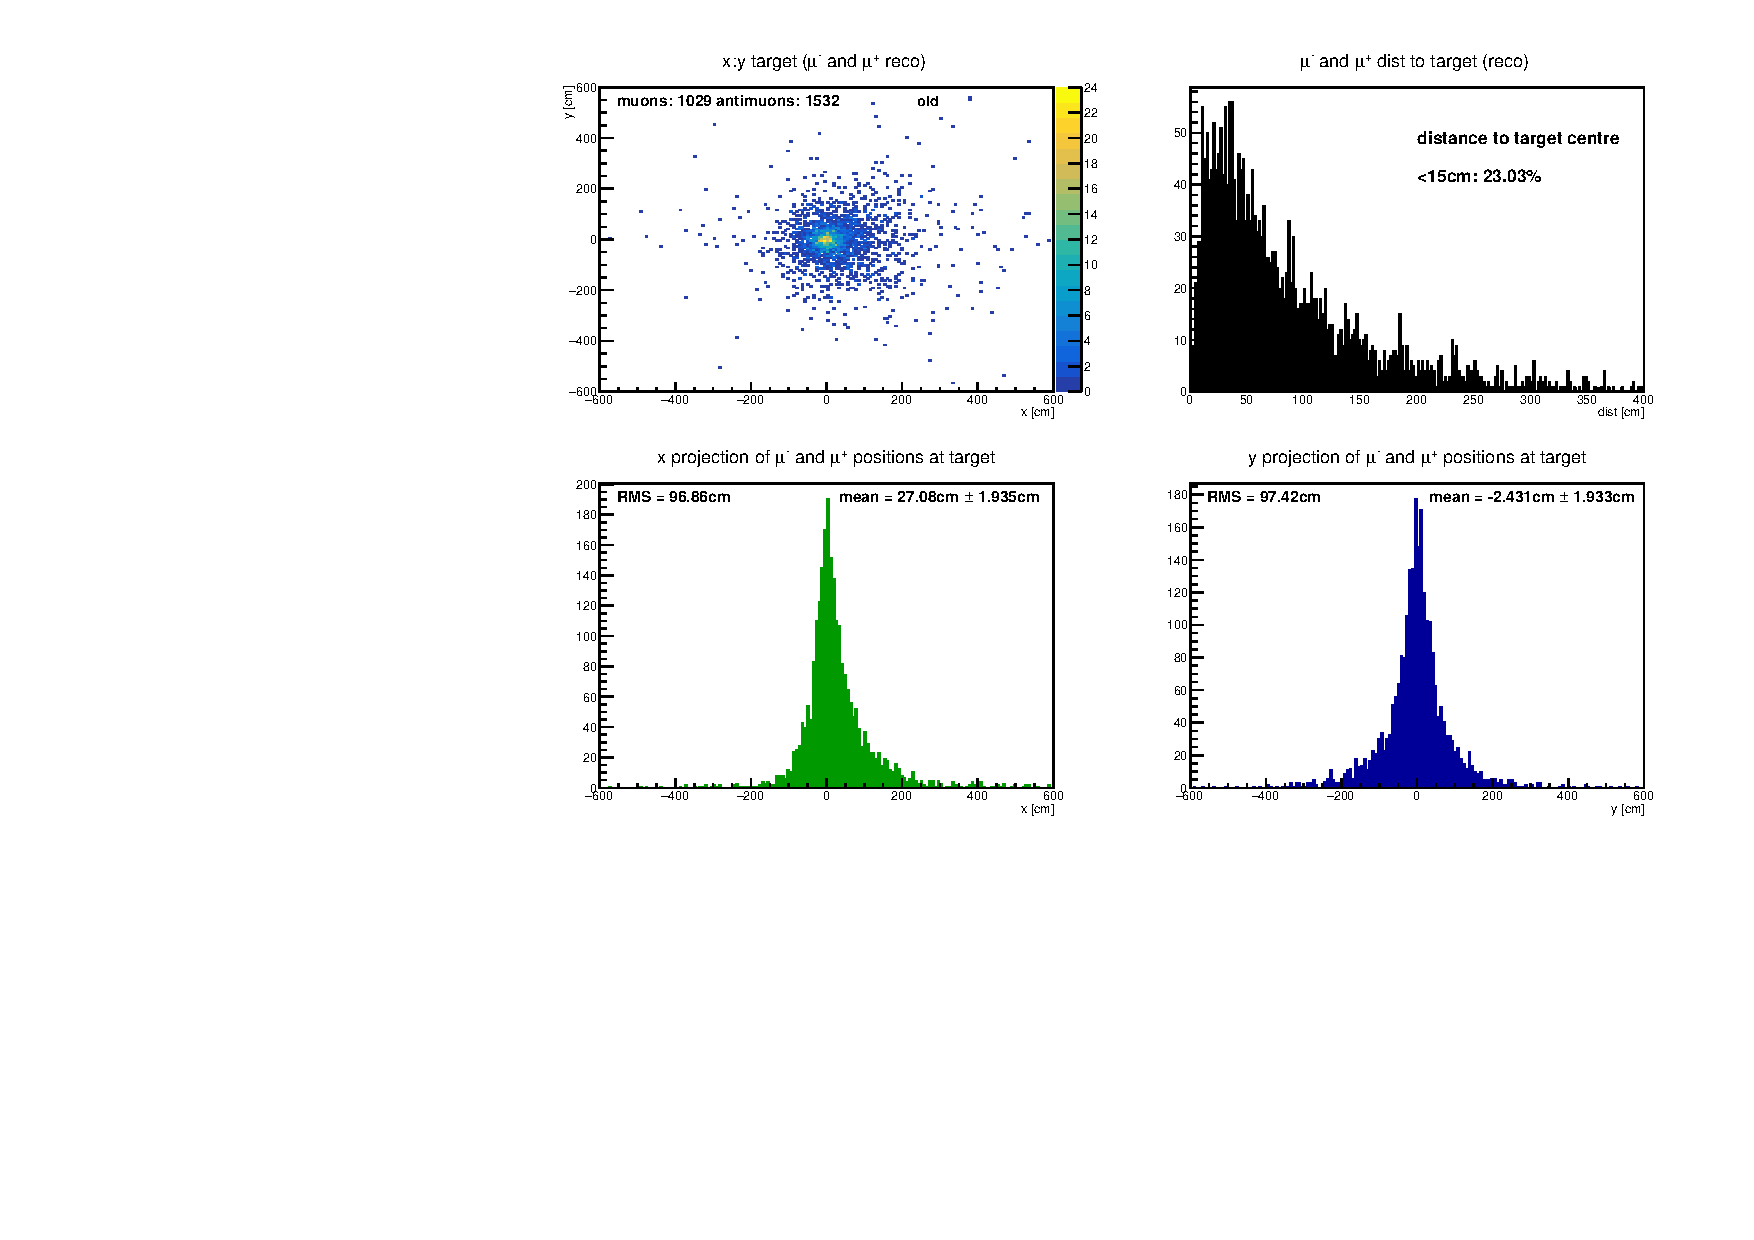
\includegraphics[width=0.78\textwidth]{../hists/nofield/old/target_dist.pdf}
  \end{figure}
\end{frame}

%------------------------------------------------------------------------------------------
\section{new data samples}
%------------------------------------------------------------------------------------------

\begin{frame}[t]{}
  \begin{figure}
    \centering
    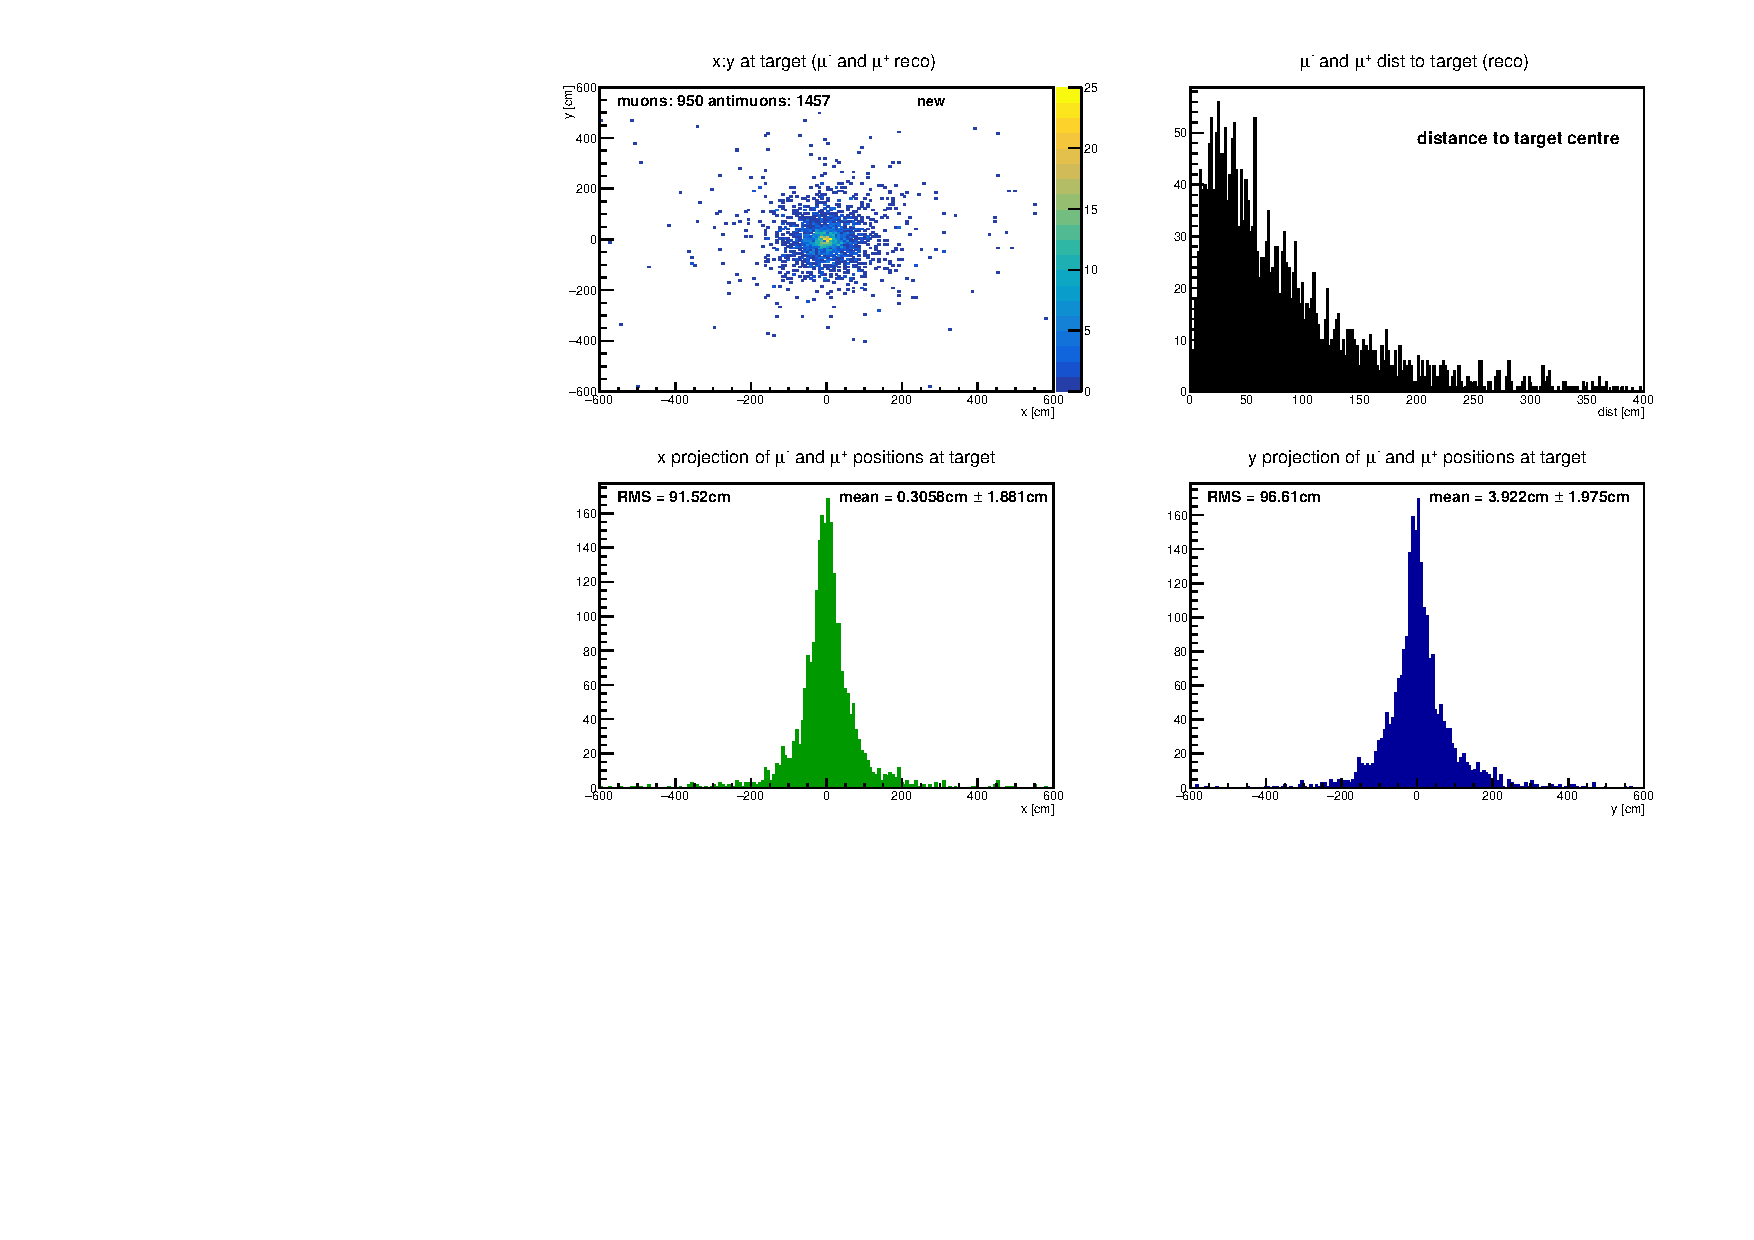
\includegraphics[width=0.78\textwidth]{../hists/nofield/new/target_dist.pdf}
  \end{figure}
\end{frame}

%------------------------------------------------------------------------------------------
\section{old data samples}
%------------------------------------------------------------------------------------------

\begin{frame}[t]{}
  \begin{figure}
    \centering
    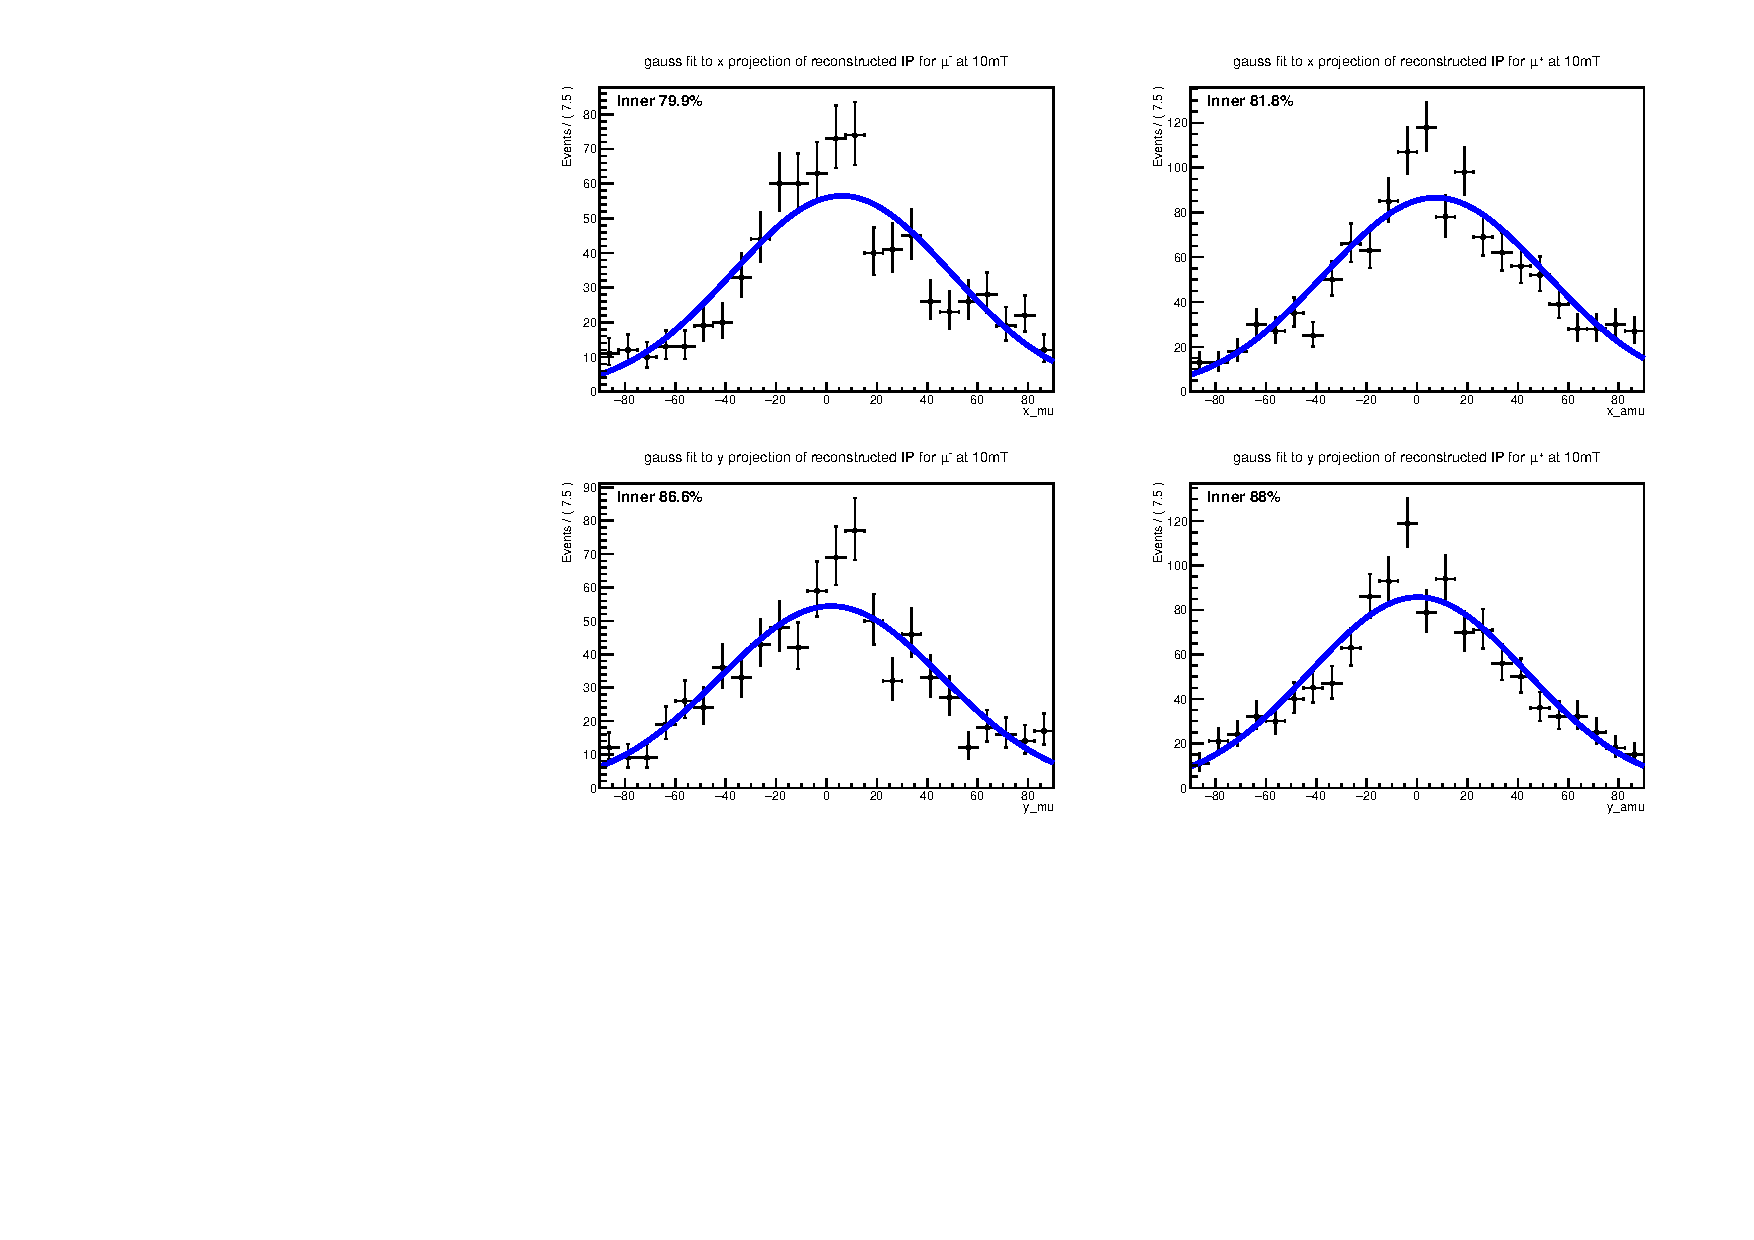
\includegraphics[width=0.78\textwidth]{../hists/nofield/old/gauss_fit.pdf}
  \end{figure}
\end{frame}

%------------------------------------------------------------------------------------------
\section{new data samples}
%------------------------------------------------------------------------------------------

\begin{frame}[t]{}
  \begin{figure}
    \centering
    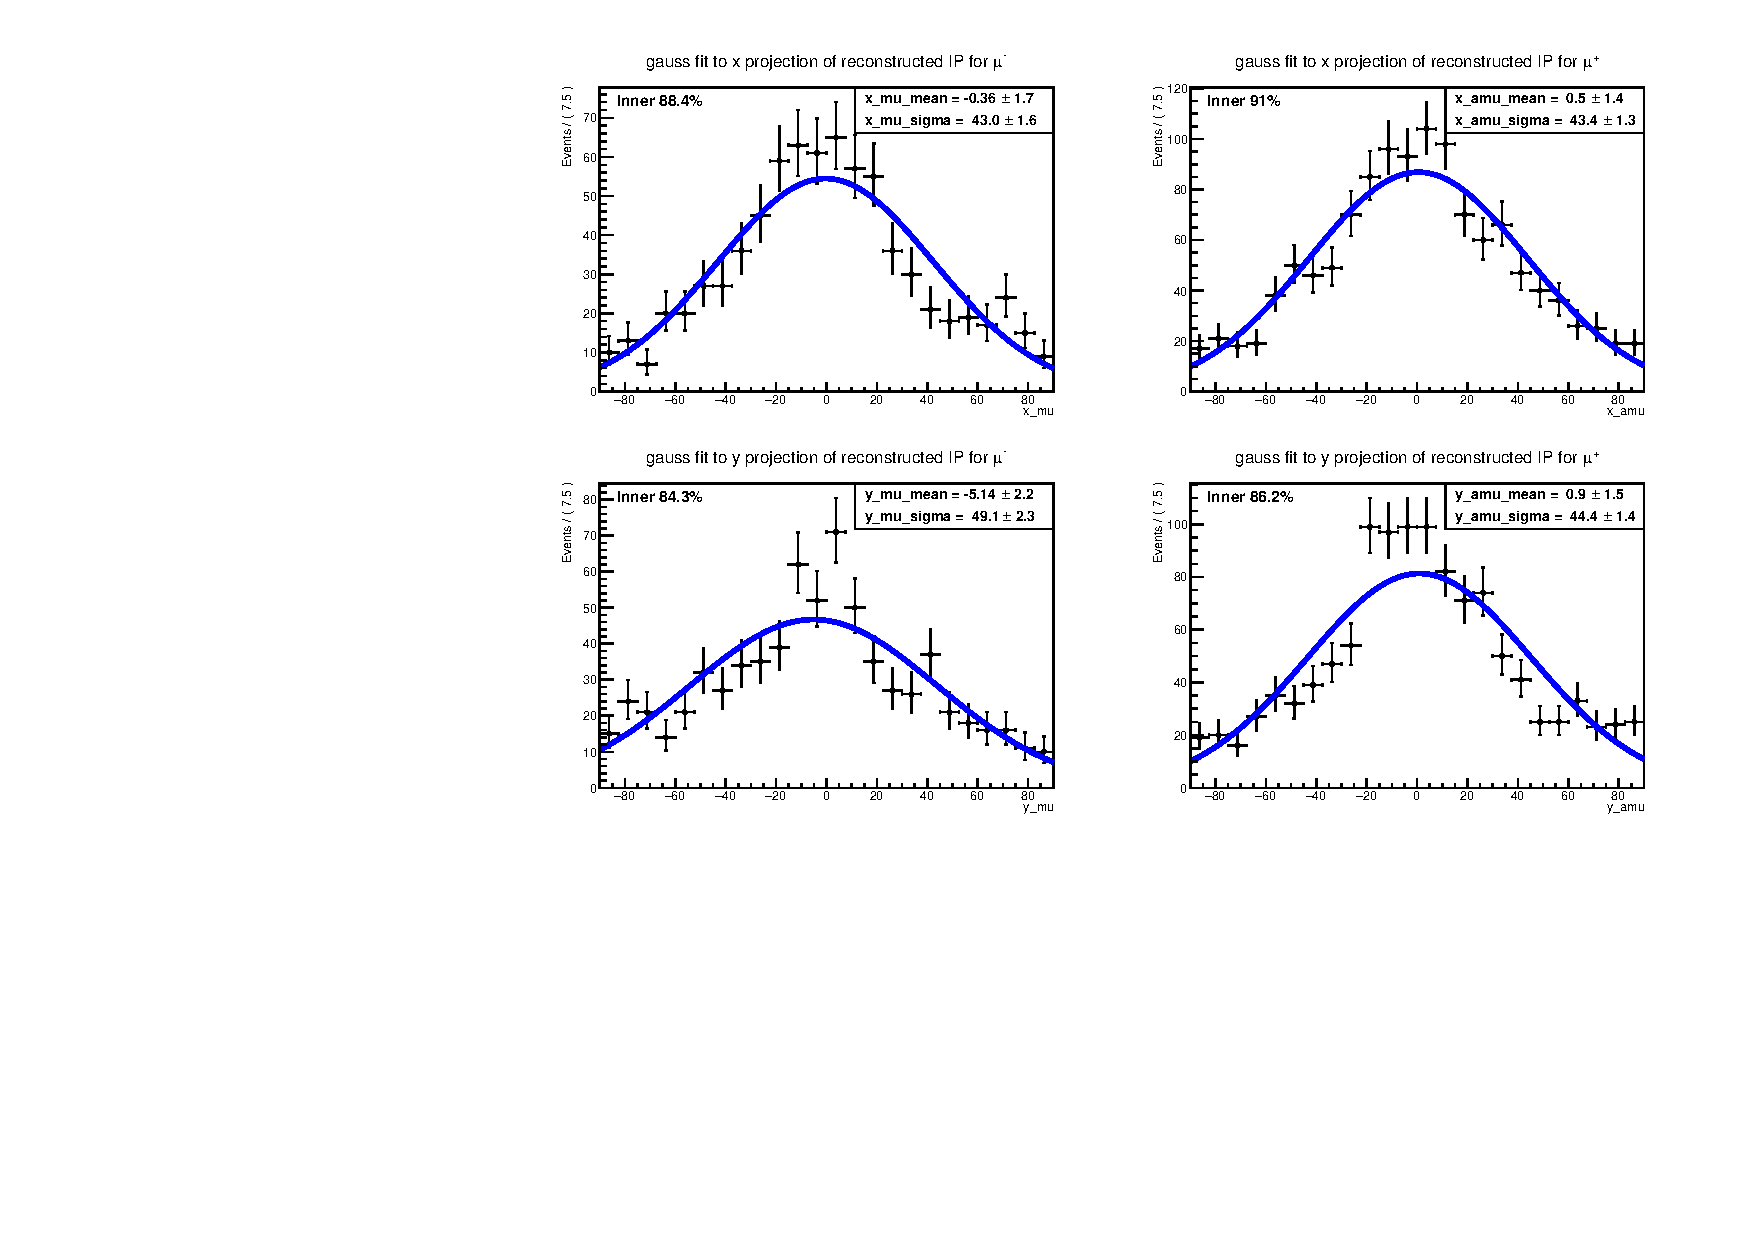
\includegraphics[width=0.78\textwidth]{../hists/nofield/new/gauss_fit.pdf}
  \end{figure}
\end{frame}

\begin{frame}[t]{comparison of old and new files}
  \begin{multicols}{2}
    \begin{figure}
      \centering
      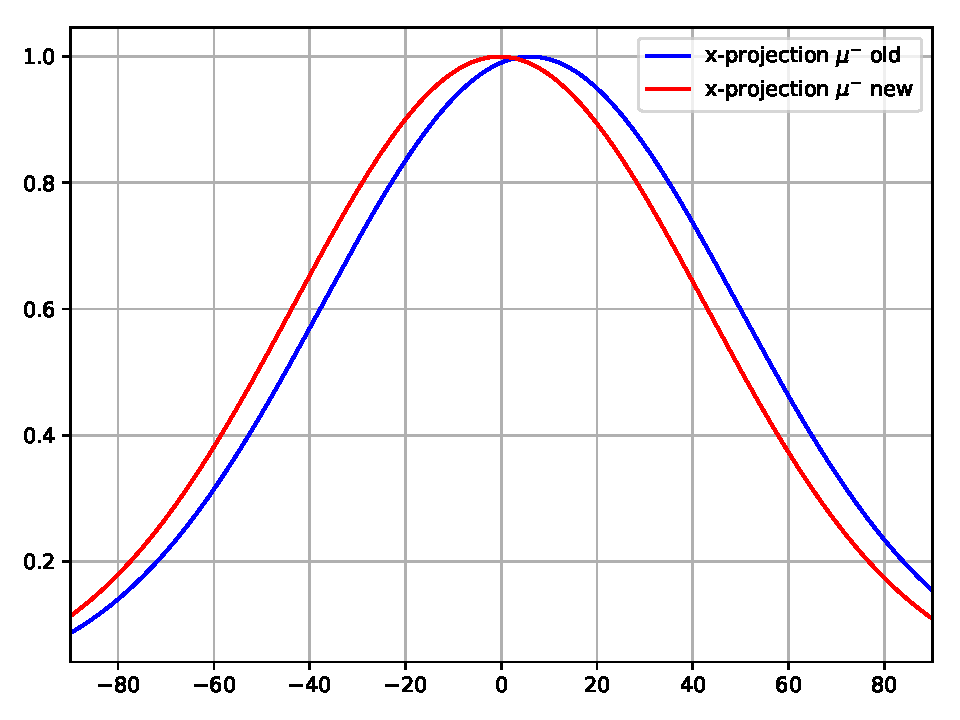
\includegraphics[width=0.5\textwidth]{../hists/nofield/comp/gauss_comparison_x-.pdf}
    \end{figure}
    \columnbreak
    \begin{figure}
      \centering
      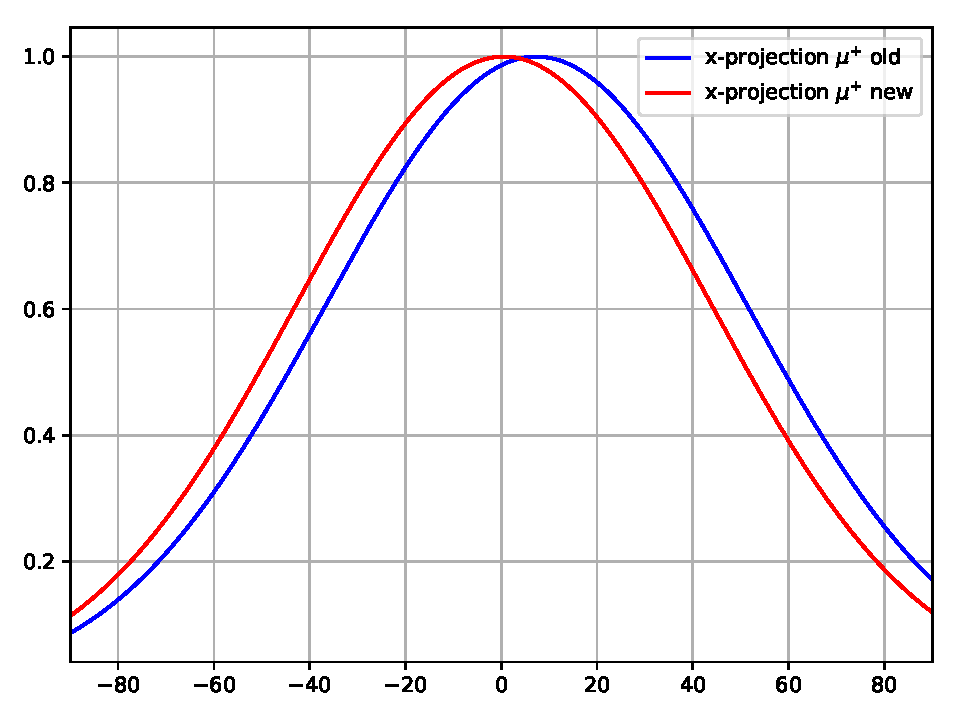
\includegraphics[width=0.5\textwidth]{../hists/nofield/comp/gauss_comparison_x+.pdf}
    \end{figure}
  \end{multicols}
\end{frame}

\begin{frame}[t]{comparison of old and new files}
  \begin{multicols}{2}
    \begin{figure}
      \centering
      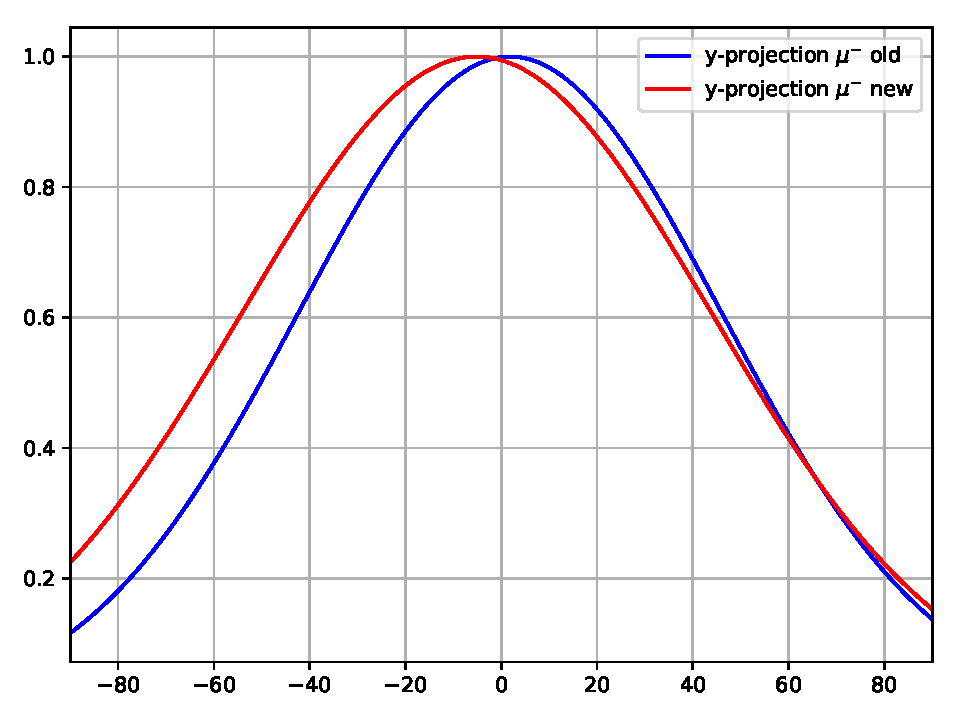
\includegraphics[width=0.5\textwidth]{../hists/nofield/comp/gauss_comparison_y-.pdf}
    \end{figure}
    \columnbreak
    \begin{figure}
      \centering
      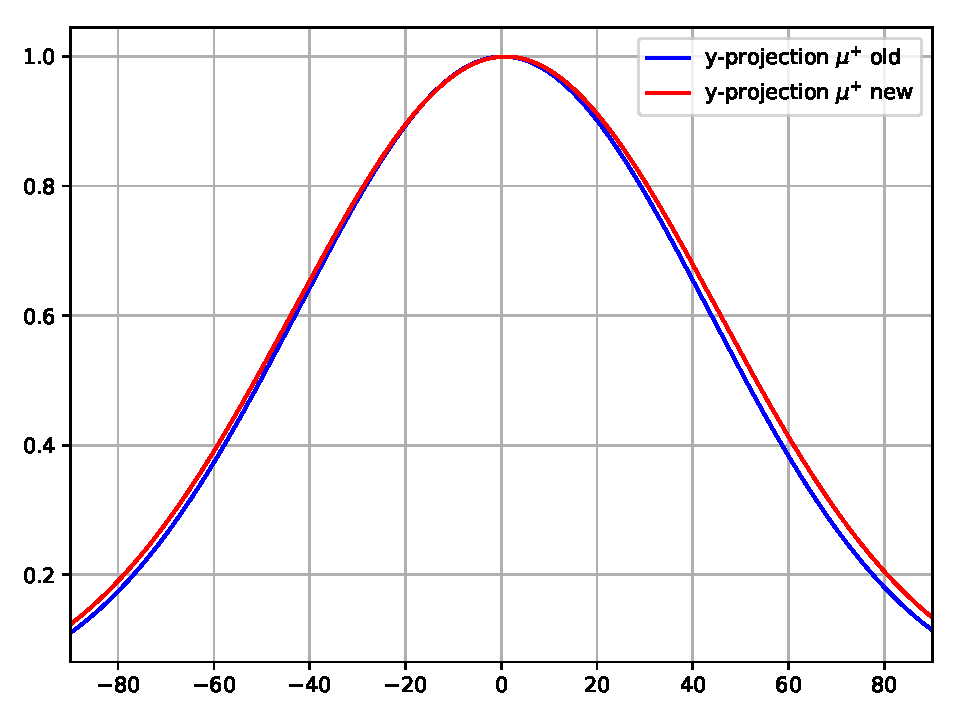
\includegraphics[width=0.5\textwidth]{../hists/nofield/comp/gauss_comparison_y+.pdf}
    \end{figure}
  \end{multicols}
\end{frame}

%------------------------------------------------------------------------------------------
\section{old data samples}
%------------------------------------------------------------------------------------------

\begin{frame}[t]{}
  \begin{figure}
    \centering
    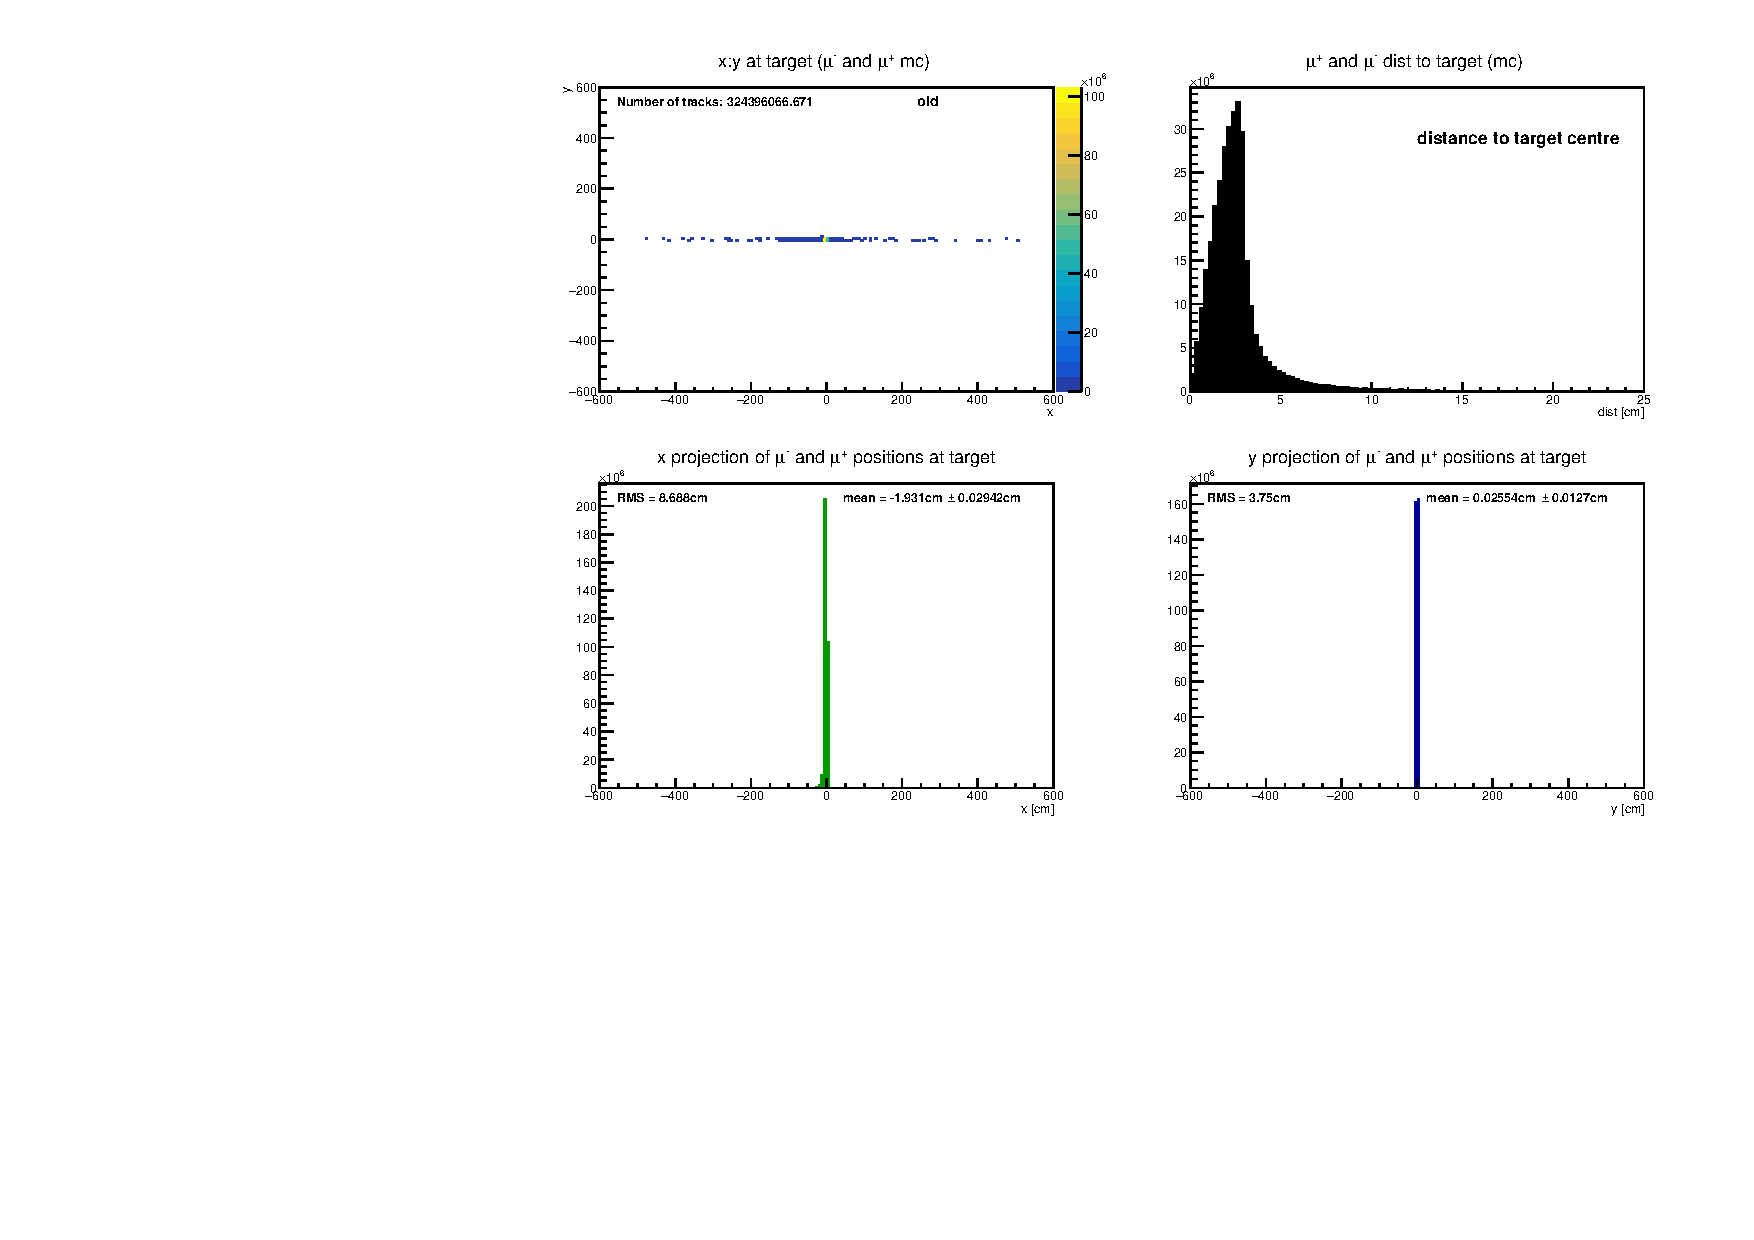
\includegraphics[width=0.78\textwidth]{../hists/nofield/old/mc_target_dist.pdf}
  \end{figure}
\end{frame}

%------------------------------------------------------------------------------------------
\section{new data samples}
%------------------------------------------------------------------------------------------

\begin{frame}[t]{}
  \begin{figure}
    \centering
    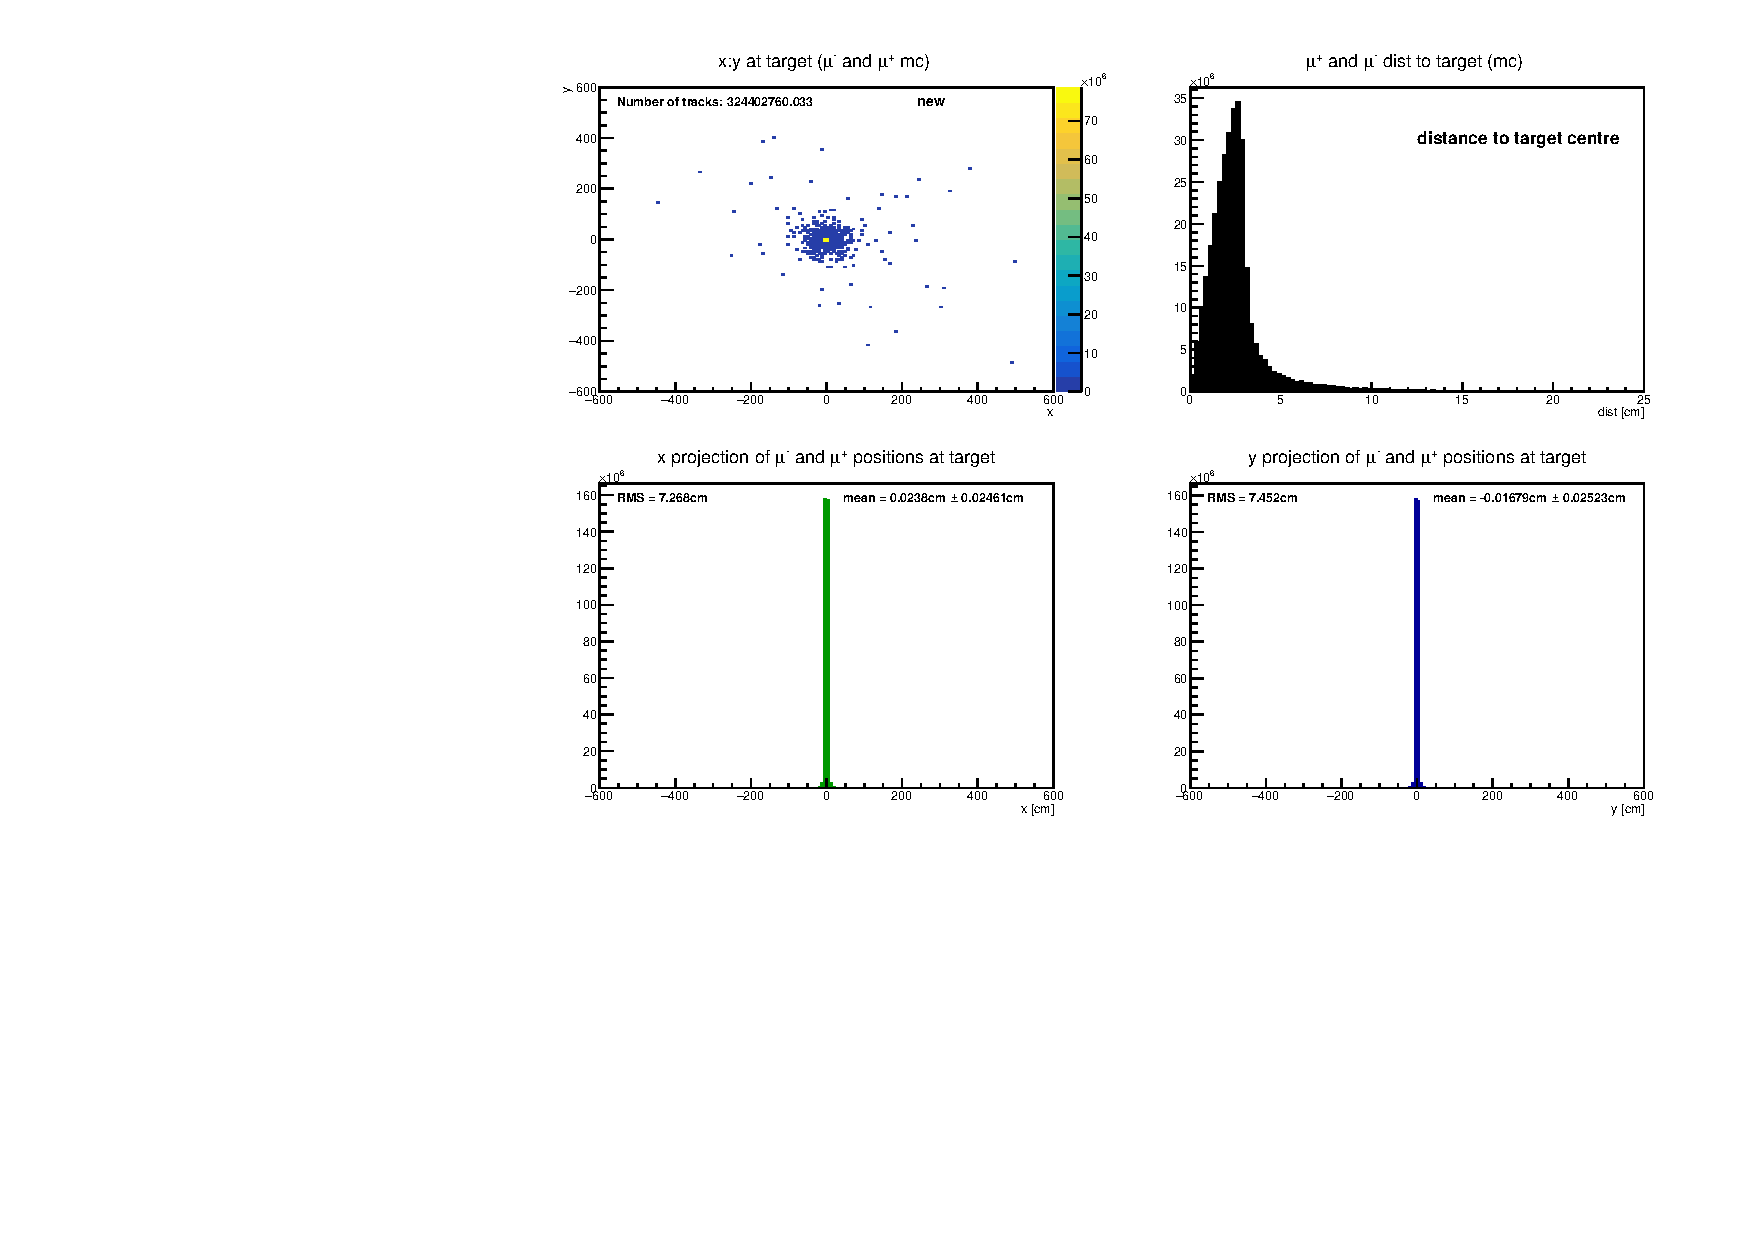
\includegraphics[width=0.78\textwidth]{../hists/nofield/new/mc_target_dist.pdf}
  \end{figure}
\end{frame}

\begin{frame}[t]{Divided for $\mu^+$ and $\mu^-$ all momenta but muon shield field = 10mT}
  \begin{multicols}{2}
    \begin{figure}
      \centering
      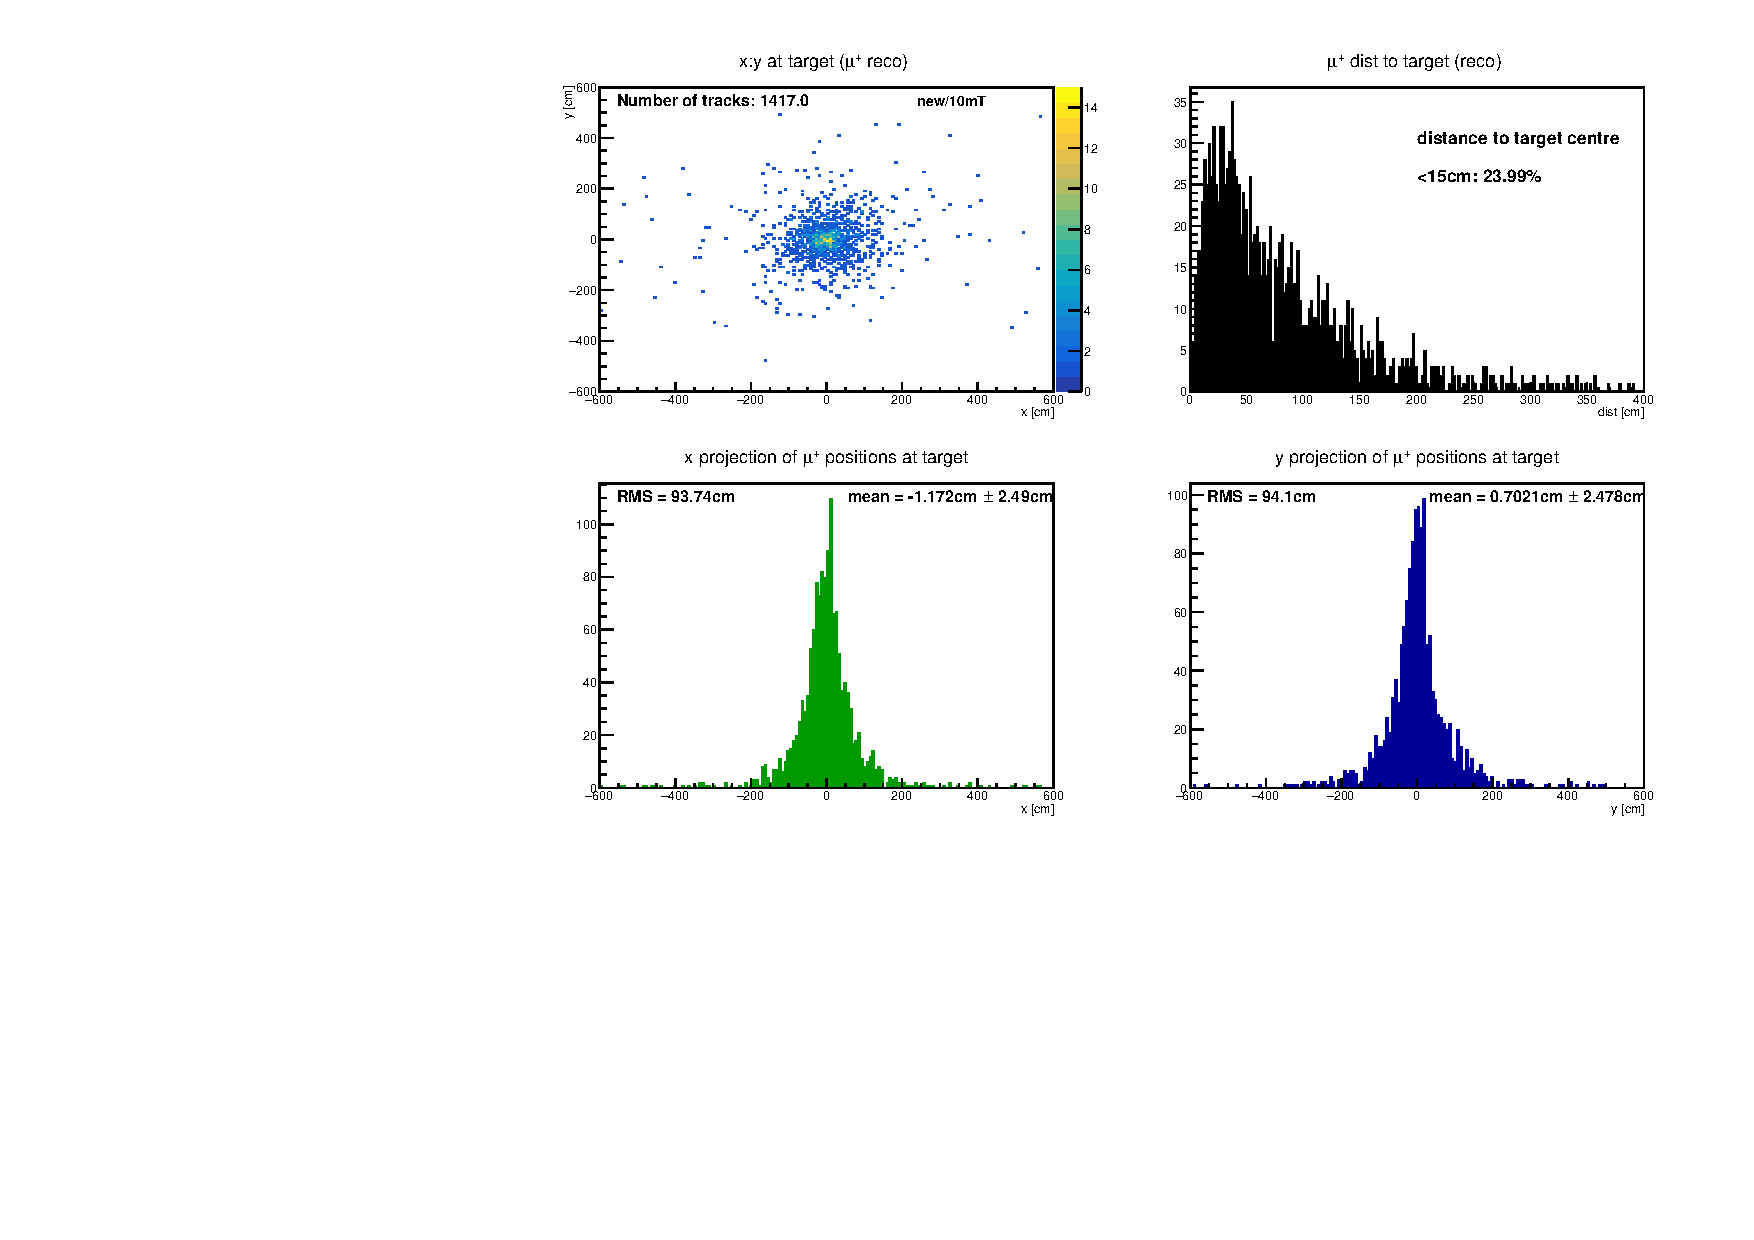
\includegraphics[width=0.5\textwidth]{../hists/nofield/new/10mT/target_dist_amu.pdf}
    \end{figure}
    \columnbreak
    \begin{figure}
      \centering
      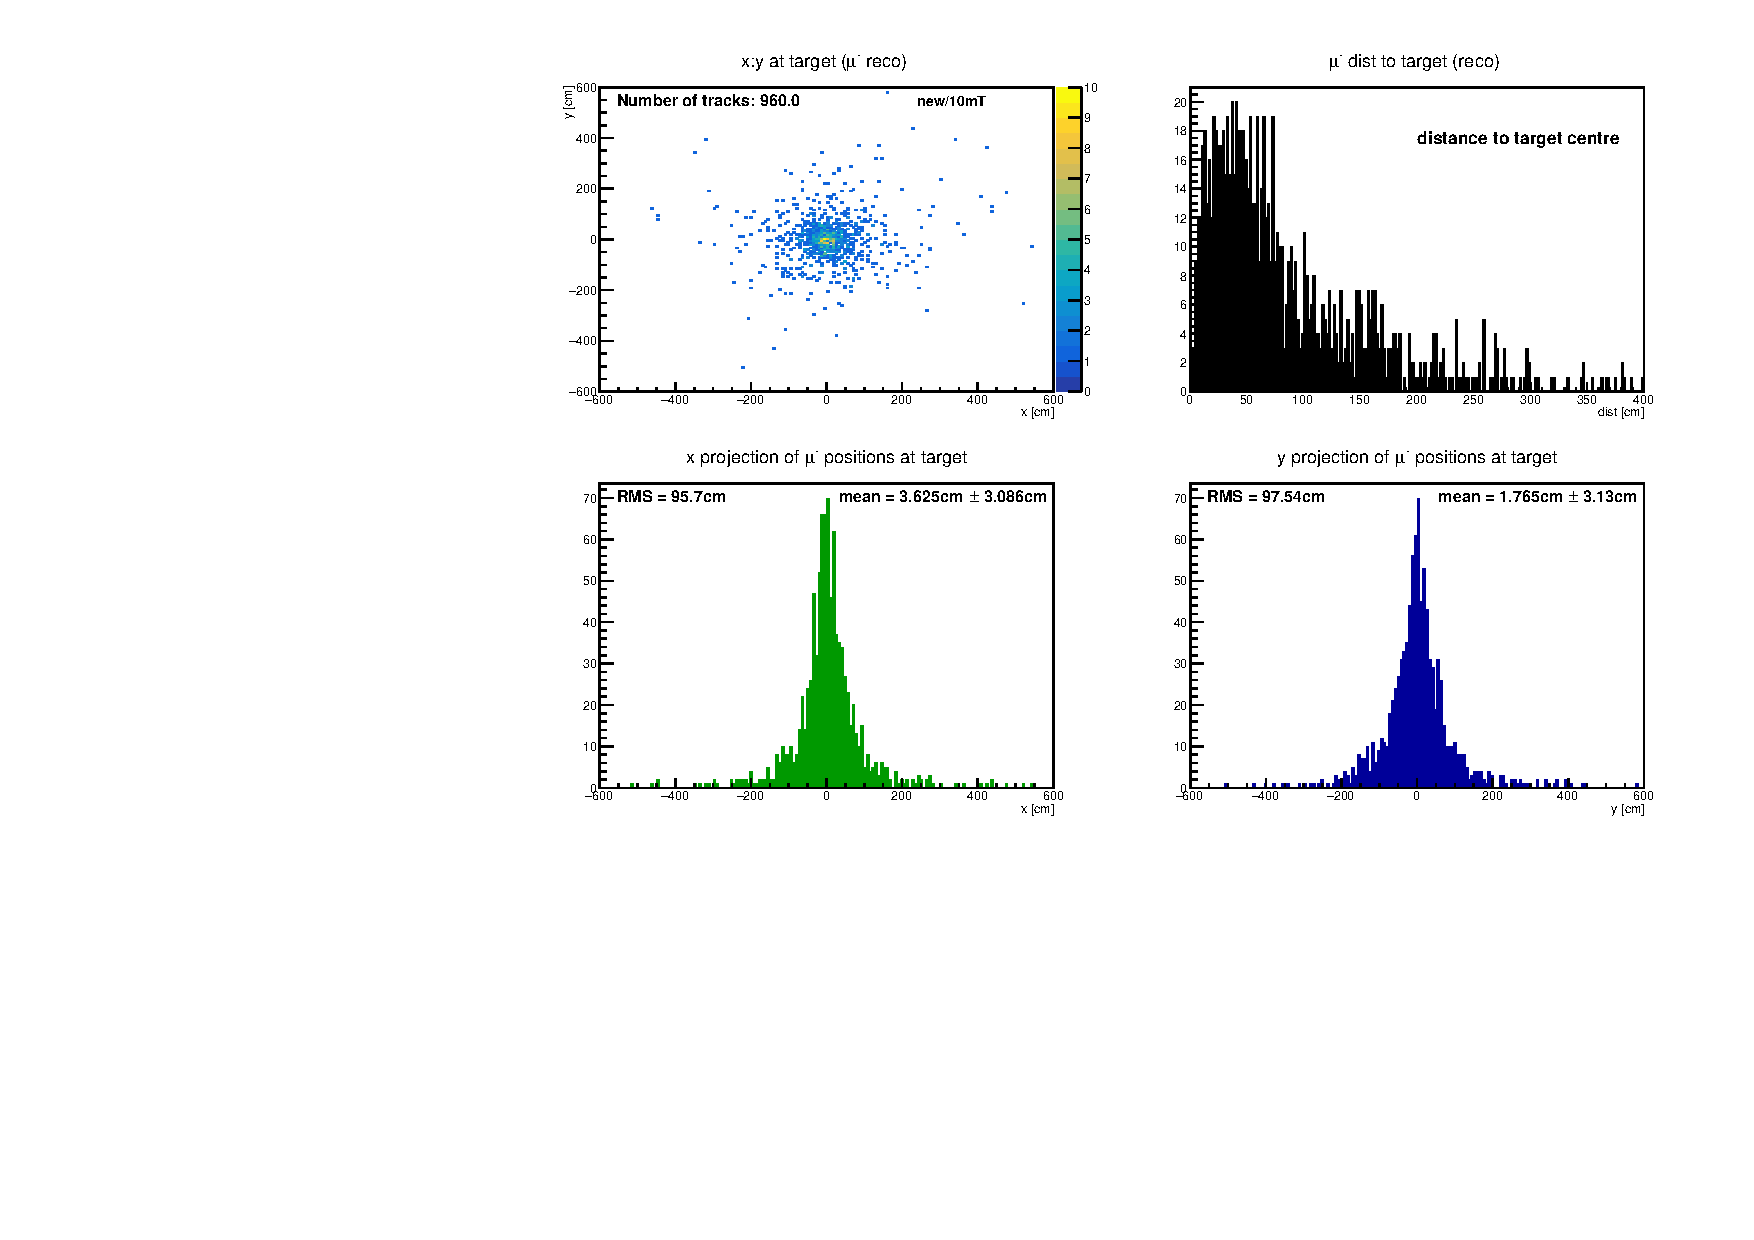
\includegraphics[width=0.5\textwidth]{../hists/nofield/new/10mT/target_dist_mu.pdf}
    \end{figure}
  \end{multicols}
\end{frame}

\begin{frame}[t]{comparison of no field and 10mT in Muon shield}
  \begin{multicols}{2}
    \begin{figure}
      \centering
      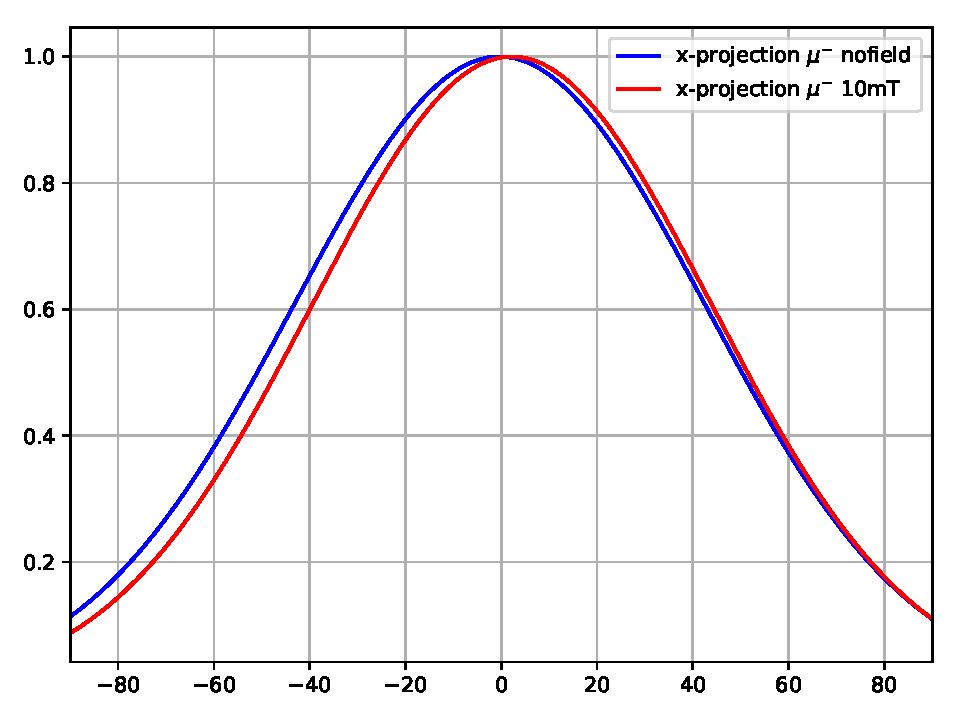
\includegraphics[width=0.5\textwidth]{../hists/nofield/comp/gauss_comparison_x-_10mT.pdf}
    \end{figure}
    \columnbreak
    \begin{figure}
      \centering
      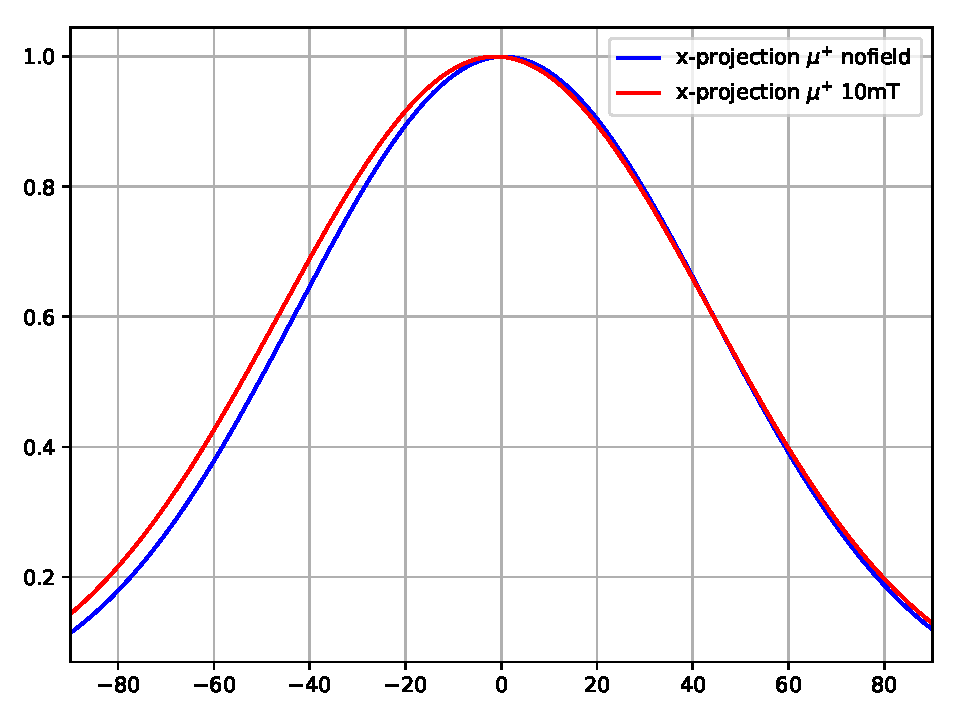
\includegraphics[width=0.5\textwidth]{../hists/nofield/comp/gauss_comparison_x+_10mT.pdf}
    \end{figure}
  \end{multicols}
\end{frame}

\begin{frame}[t]{comparison of no field and 10mT in Muon shield}
  \begin{multicols}{2}
    \begin{figure}
      \centering
      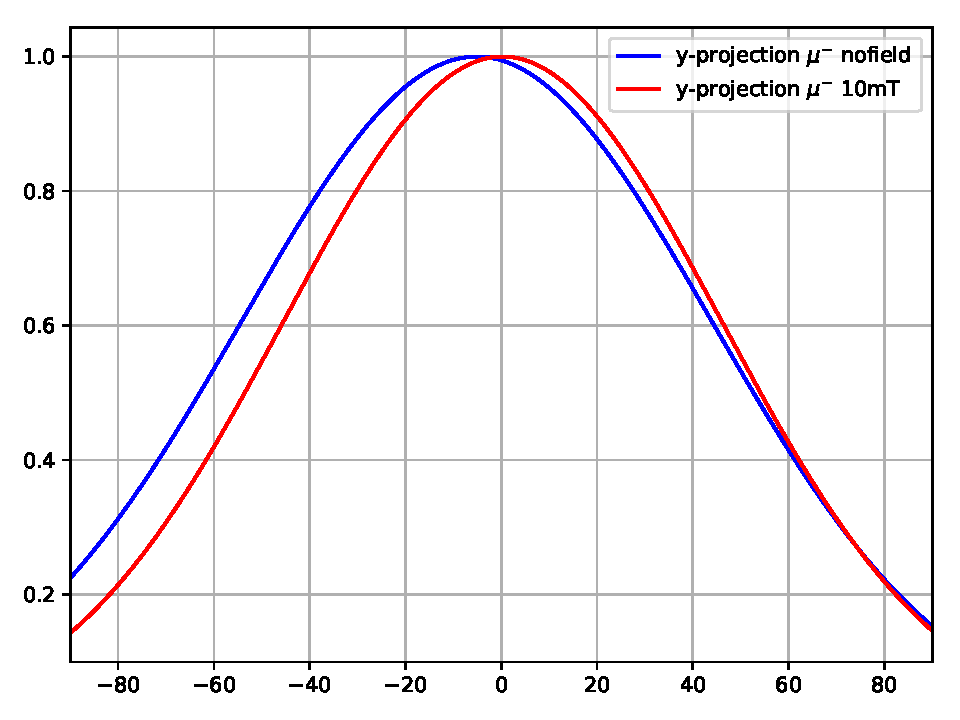
\includegraphics[width=0.5\textwidth]{../hists/nofield/comp/gauss_comparison_y-_10mT.pdf}
    \end{figure}
    \columnbreak
    \begin{figure}
      \centering
      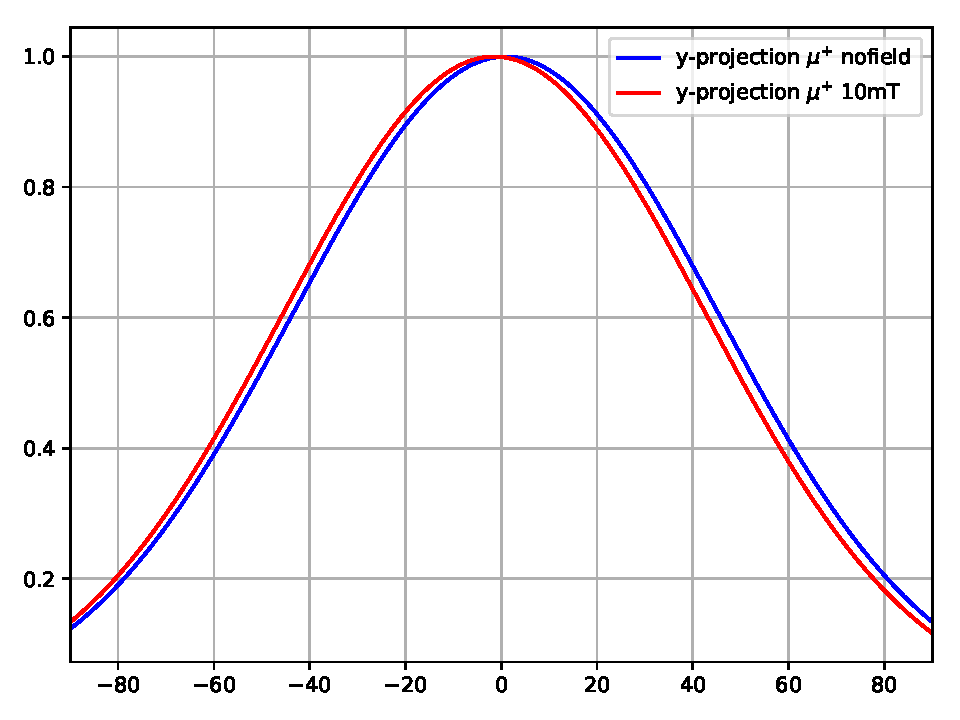
\includegraphics[width=0.5\textwidth]{../hists/nofield/comp/gauss_comparison_y+_10mT.pdf}
    \end{figure}
  \end{multicols}
\end{frame}

\begin{frame}
  \begin{table}
    \centering
    \begin{tabular}{c
                    S
                    S}
      \toprule
      {$\mu^{+}$} & {$B_\text{mu shield}=\SI{10}{\milli\tesla}$} & {$B_\text{mu shield}=\SI{0}{\tesla}$} \\
      \midrule
      mean $x$ /cm & -1.16(150) & 0.512(1394)  \\
      mean $y$ /cm & -1.45(147)   & 0.911(1477)  \\
      $\sigma_x$ /cm & 45.03(146)       & 43.40(132)  \\
      $\sigma_y$ /cm & 44.13(141)      & 44.43(142) \\
      \midrule
      {$\mu^{-}$} & {$B_\text{mu shield}=\SI{10}{\milli\tesla}$} & {$B_\text{mu shield}=\SI{0}{\tesla}$} \\
      \midrule
      mean $x$ /cm & 2.215(1658) & -0.363(1741)    \\
      mean $y$ /cm & 0.281(1908) & -5.136(2199)   \\
      $\sigma_x$ /cm & 41.76(152)   & 42.965(1630)   \\
      $\sigma_y$ /cm & 45.72(188)   & 49.077(2296)   \\
      \bottomrule
    \end{tabular}
    \caption{Means and sigmas of the reconstructed IP for no magnetic field and a $\SI{10}{\milli\tesla}$ field in the muon shield.}
    \label{tab:mean}
  \end{table}
\end{frame}

%%------------------------------------------------------------------------------------------
%\section{MC truth and Particle dist.}
%%------------------------------------------------------------------------------------------
%
%
%\begin{frame}[t]{Accuracy of simple linear fit to target}
%  \begin{figure}
%    \centering
%    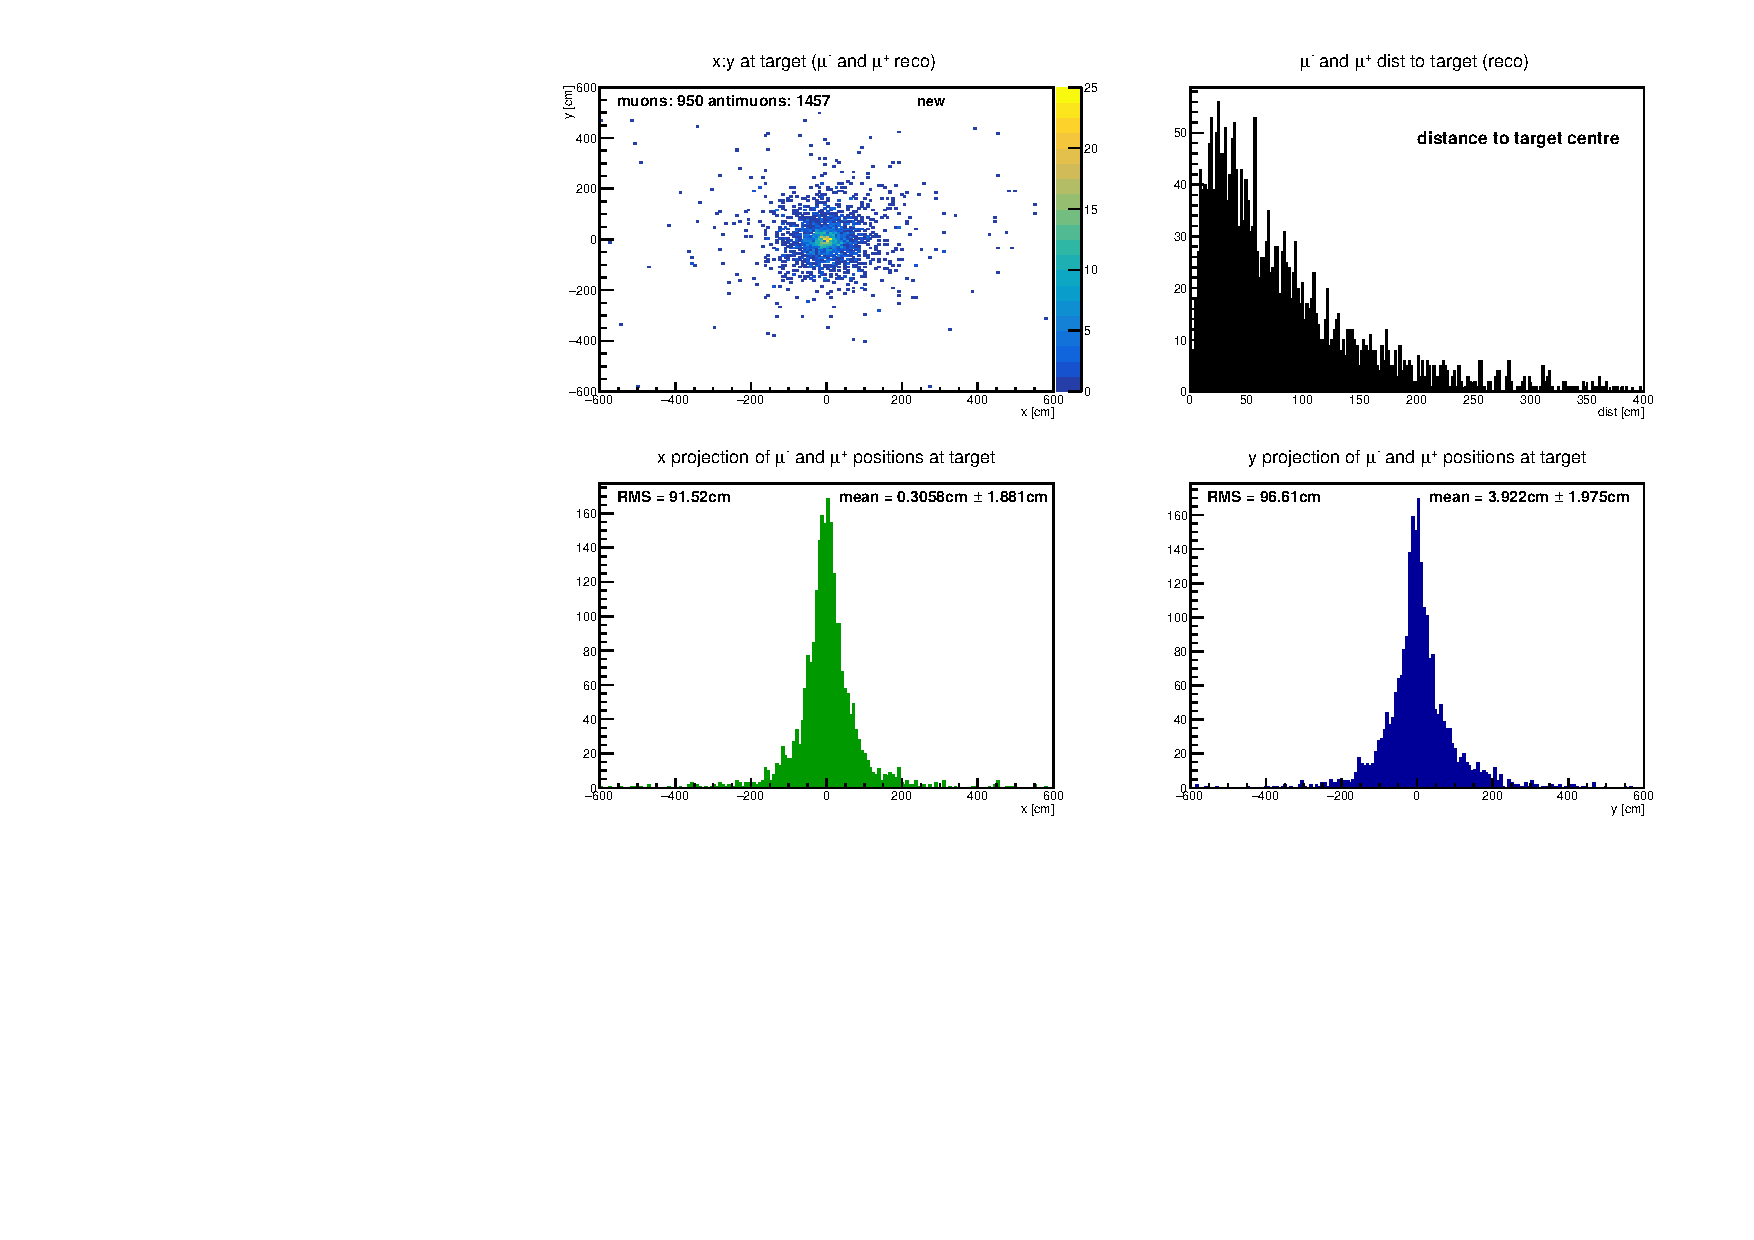
\includegraphics[width=0.65\textwidth]{../hists/nofield/new/target_dist.pdf}
%  \end{figure}
%\end{frame}

%\begin{frame}[t]{Accuracy of extrapolation to $z=0$ and linear fit to target}
%  \begin{figure}
%    \centering
%    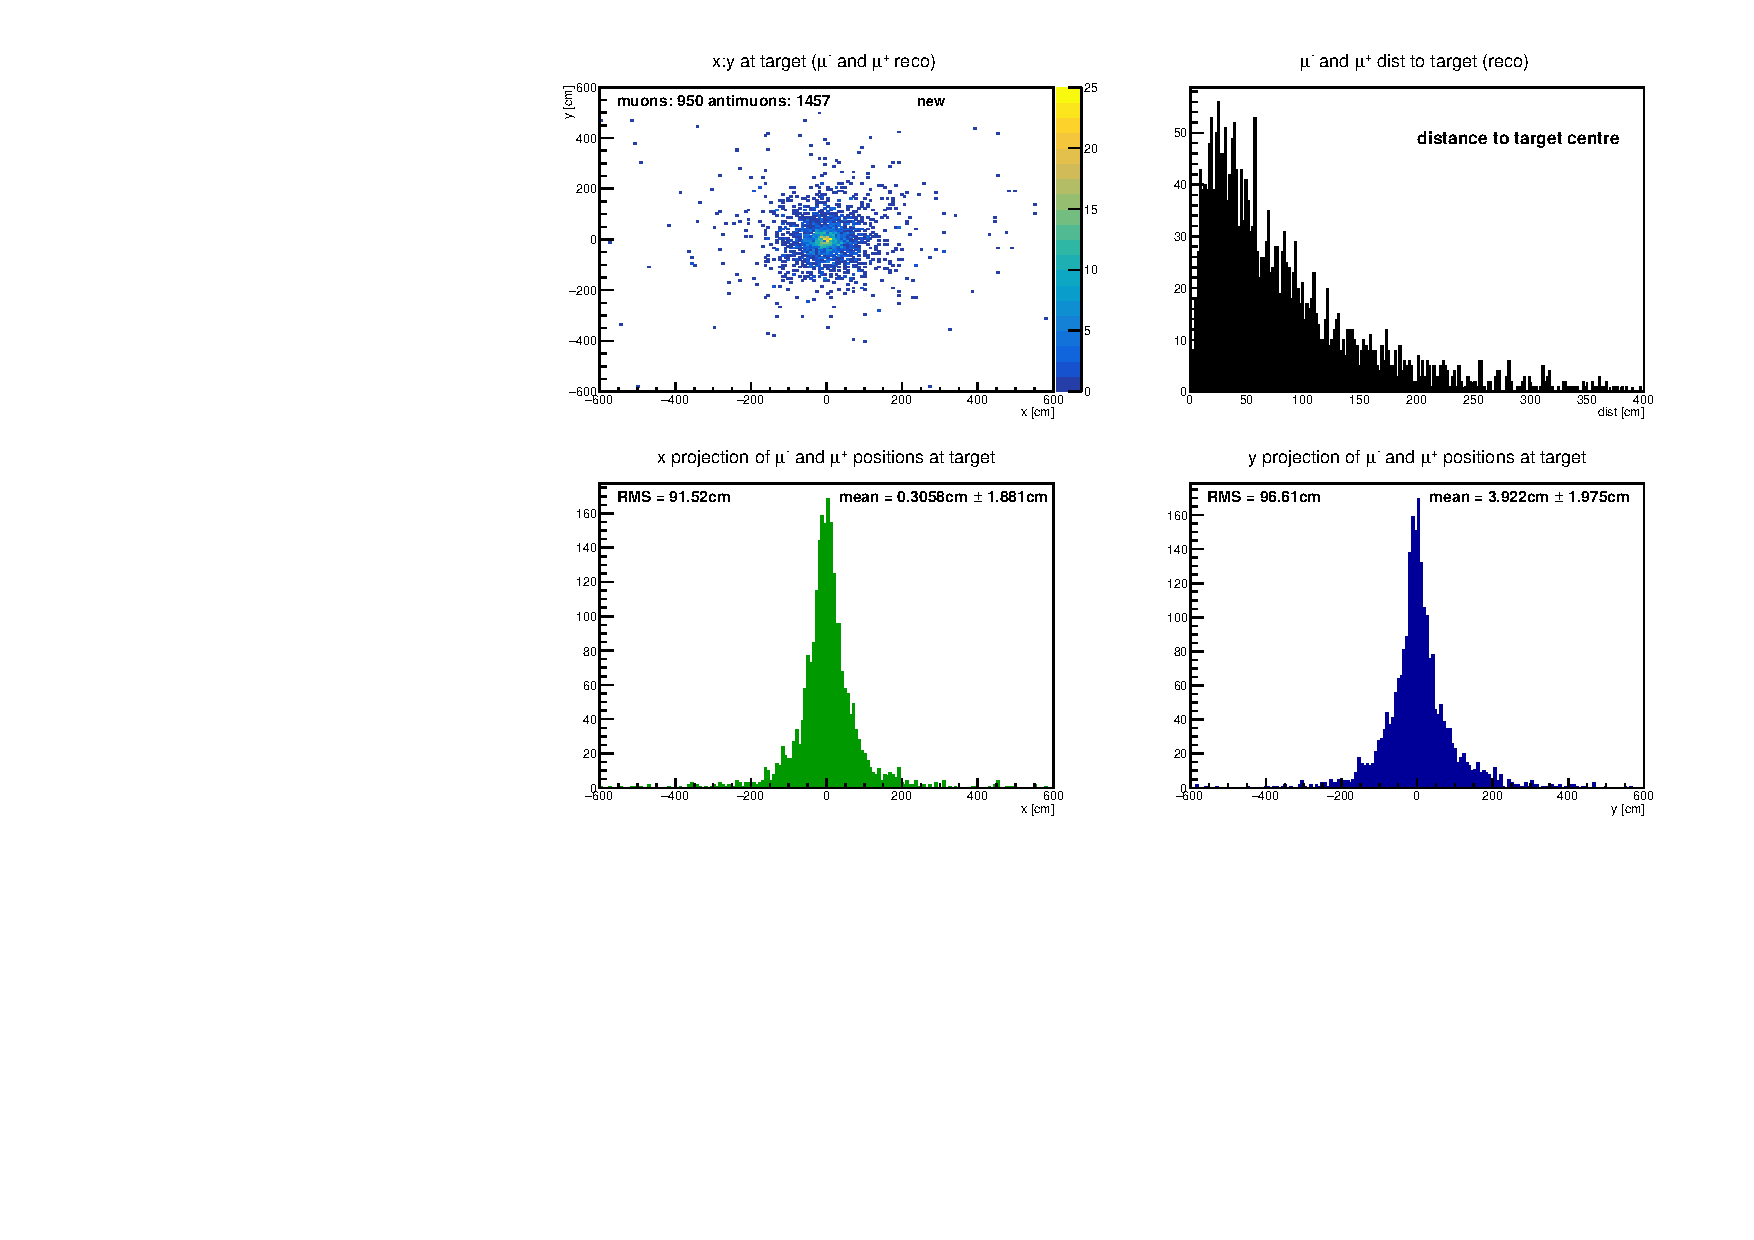
\includegraphics[width=0.65\textwidth]{../hists/nofield/new/target_dist.pdf}
%  \end{figure}
%\end{frame}

%------------------------------------------------------------------------------------------
\section{Particle flux in T1}
%------------------------------------------------------------------------------------------

\begin{frame}[t]
  \vspace*{\fill}
    \centering
    {\huge Investigation of particle flux in T1}
  \vspace*{\fill}
\end{frame}

\begin{frame}[t]{Investigation of particle flux in T1}
  \vspace*{\fill}
    \begin{itemize}
      \item 4 strawtube stations in SHiP
      \item each one consists of 8 planes that are made of 2 layers of strawtubes
      \item 568 straws per layer $\rightarrow$ $\num{1136}$ straws per plane $\rightarrow$ $\num{9088}$ straws per station
      \item data samples with \texttt{--MuonBack} but without \texttt{--FollowMuon} to get total flux
      \item turned \textbf{off} the magnet of $\tau$-station ($\SI{1.5}{\tesla}$) and the \texttt{EMuMagnet} ($\SI{1.0}{\tesla}$)
    \end{itemize}
  \vspace*{\fill}
\end{frame}
\begin{frame}[t]{Investigation of particle flux in T1}
  \vspace*{\fill}
    To get the total flux per spill:
    \begin{itemize}
      \item apply Monte Carlo \textbf{weights} (\num{2571} or \num{4975}) on the events.
      \item only $\num{100000}$ events, so additional factor $\frac{\num{17786274}}{\num{100000}}$ to get to the $\num{17786274}$ events of the used file \texttt{/eos/ship/data/Mbias/pythia8\_Geant4-withCharm\_onlyMuons\_4magTarget.root}.
      \item count \texttt{strawtubesPoint} hits in range of first plane (arbitrary choice) so between $z=2580$ and $z=2581.5$.
    \end{itemize}
  \vspace*{\fill}
\end{frame}

\begin{frame}[t]{}
  \begin{figure}
    \centering
    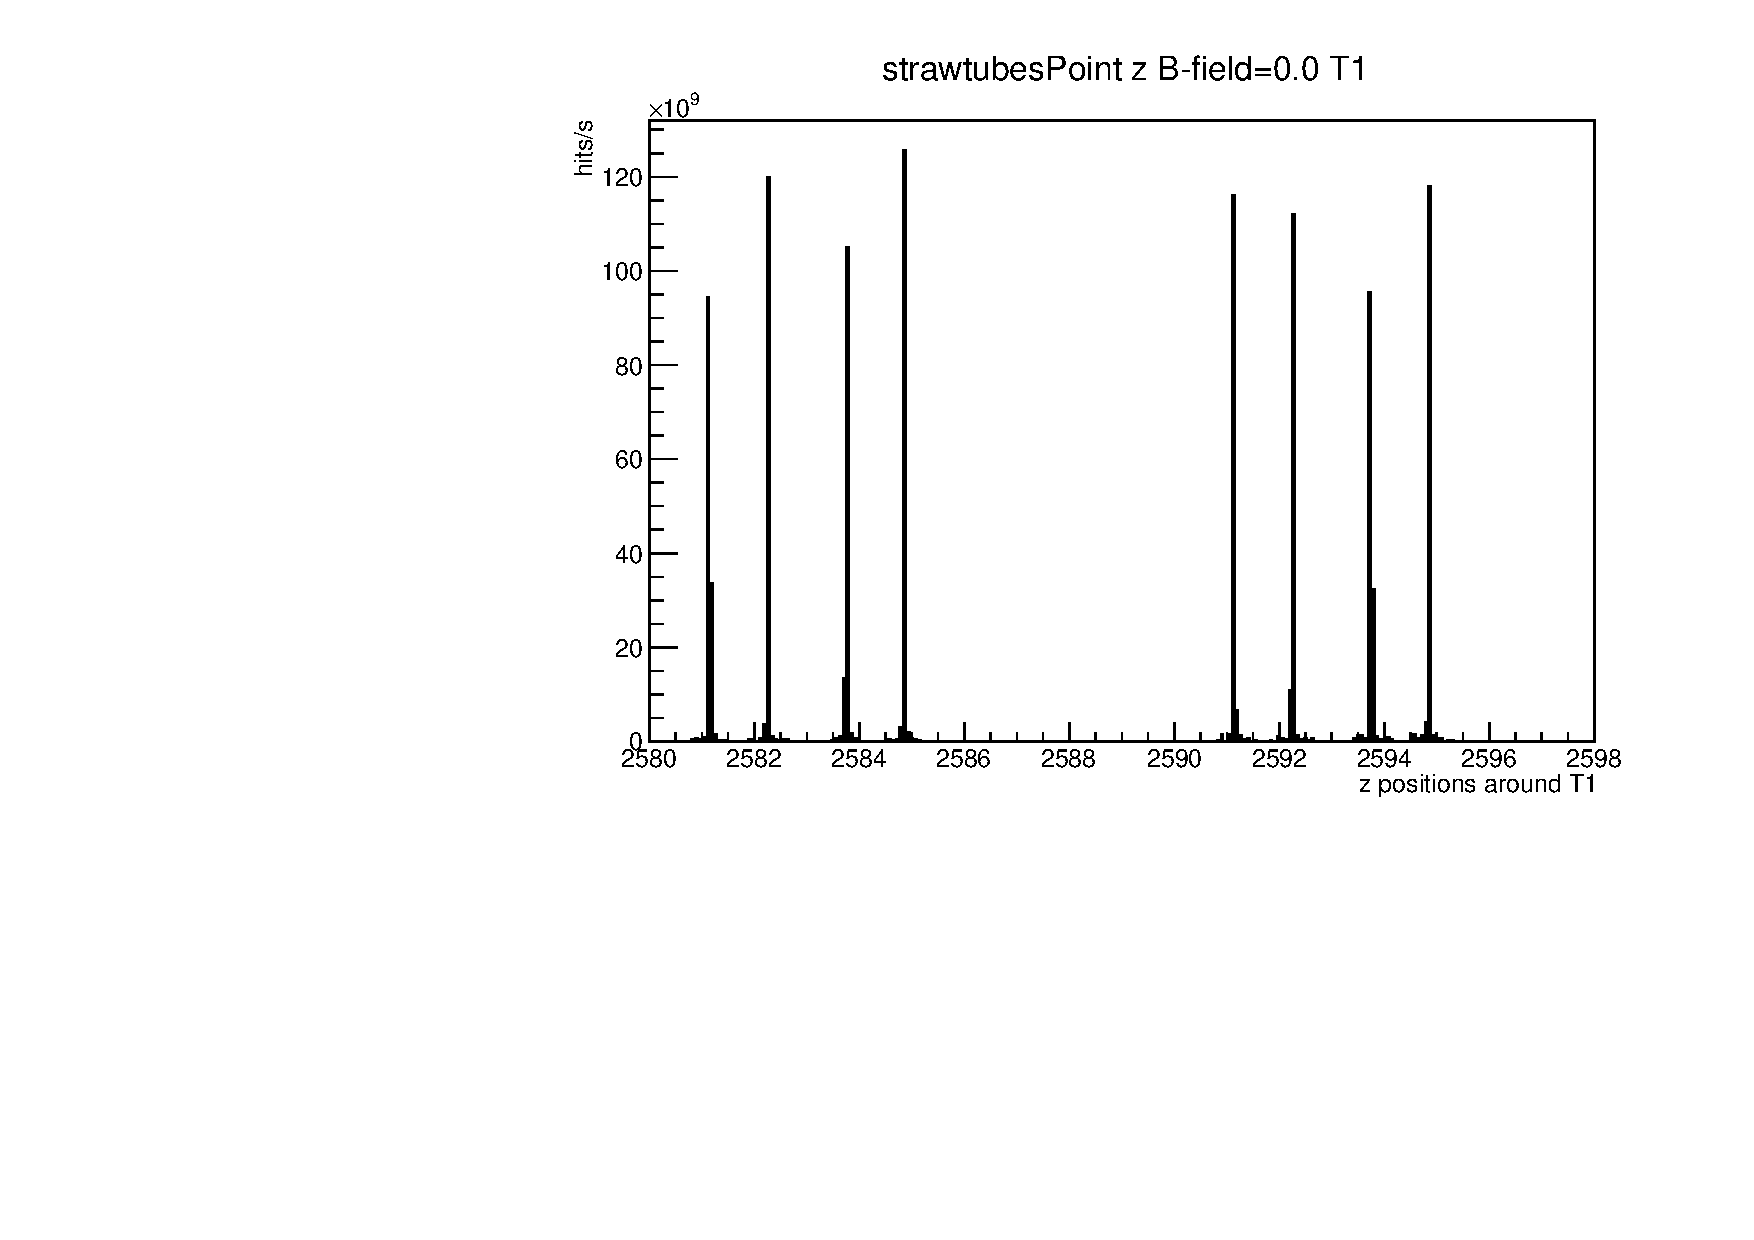
\includegraphics[width=0.78\textwidth]{../hists/strawtubes/all/z_T1.pdf}
  \end{figure}
\end{frame}

\begin{frame}[t]{}
  \begin{figure}
    \centering
    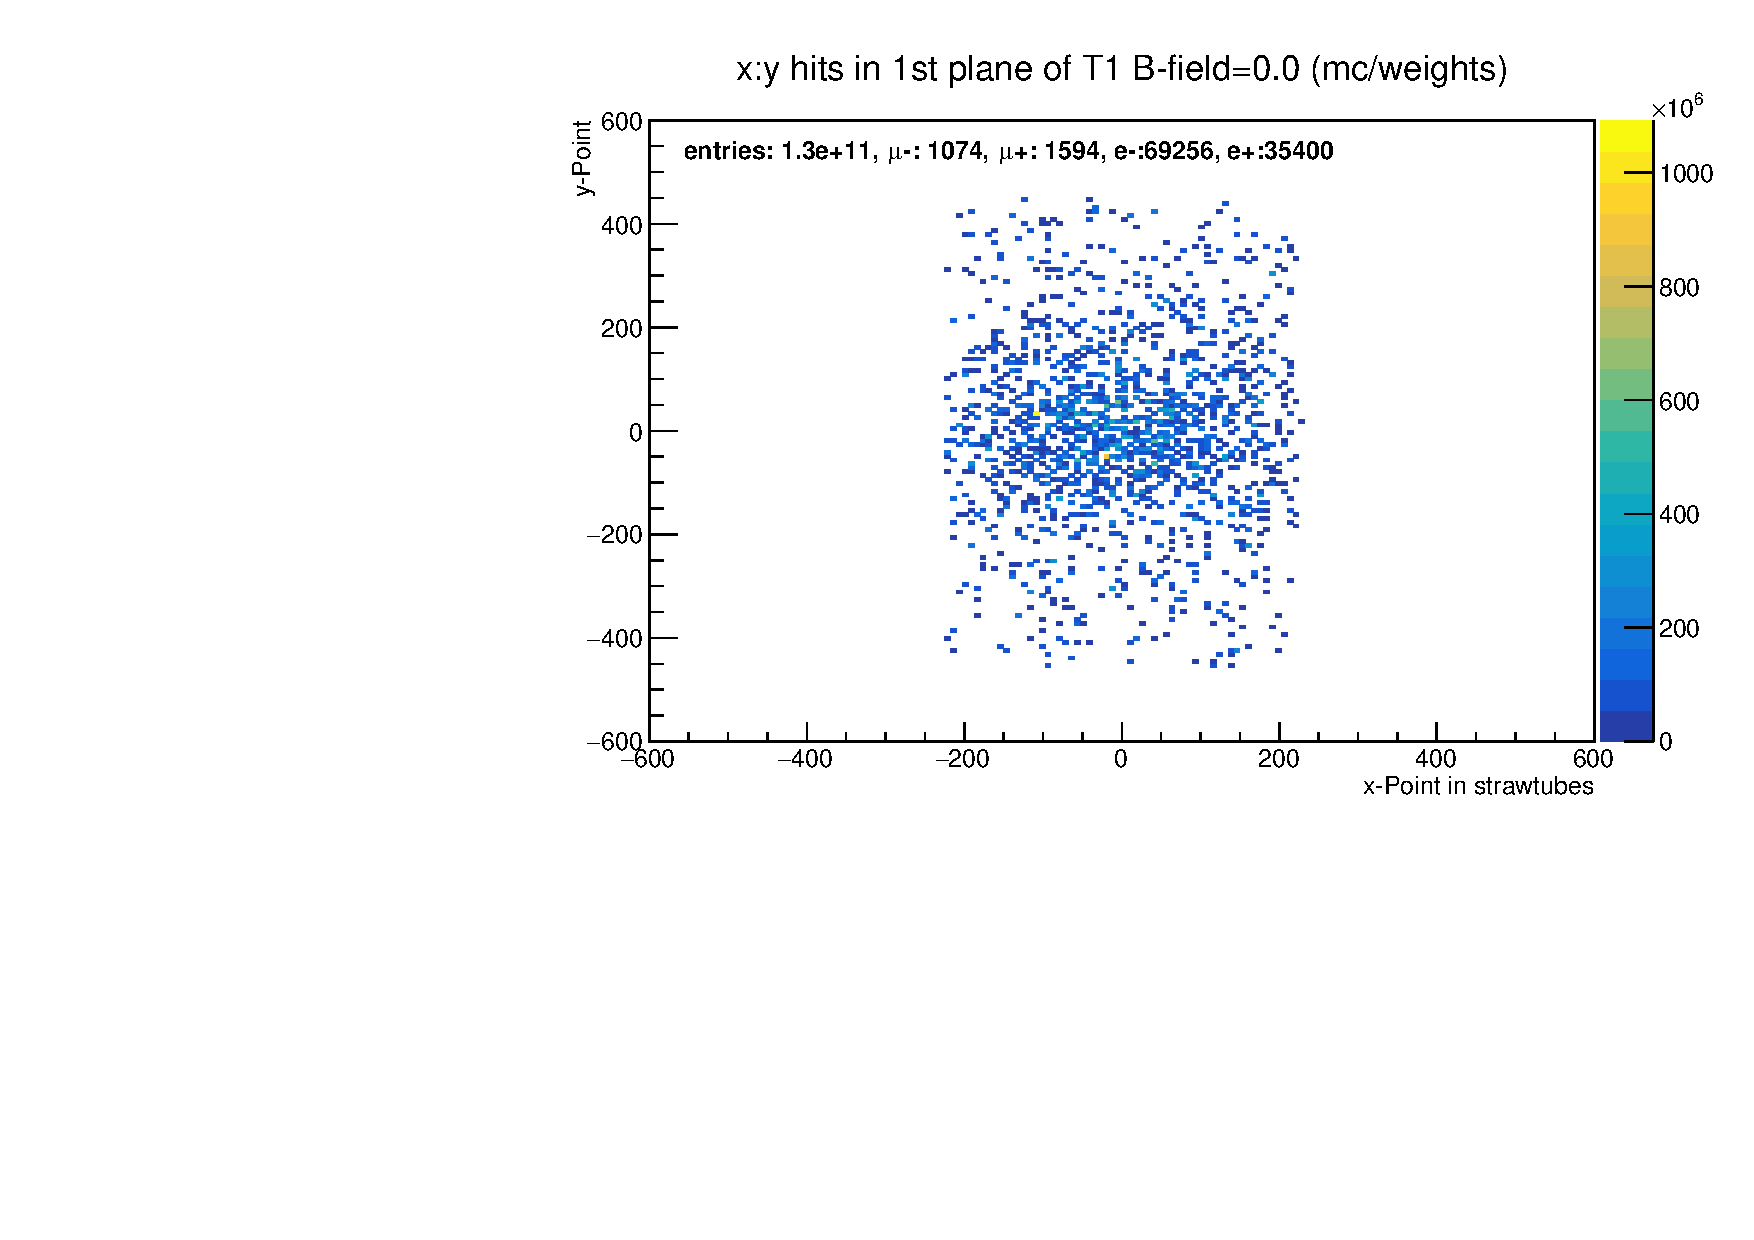
\includegraphics[width=0.78\textwidth]{../hists/strawtubes/all/xy_0.pdf}
  \end{figure}
\end{frame}

\begin{frame}[t]{}
  \vspace*{\fill}
    \begin{figure}
      \centering
      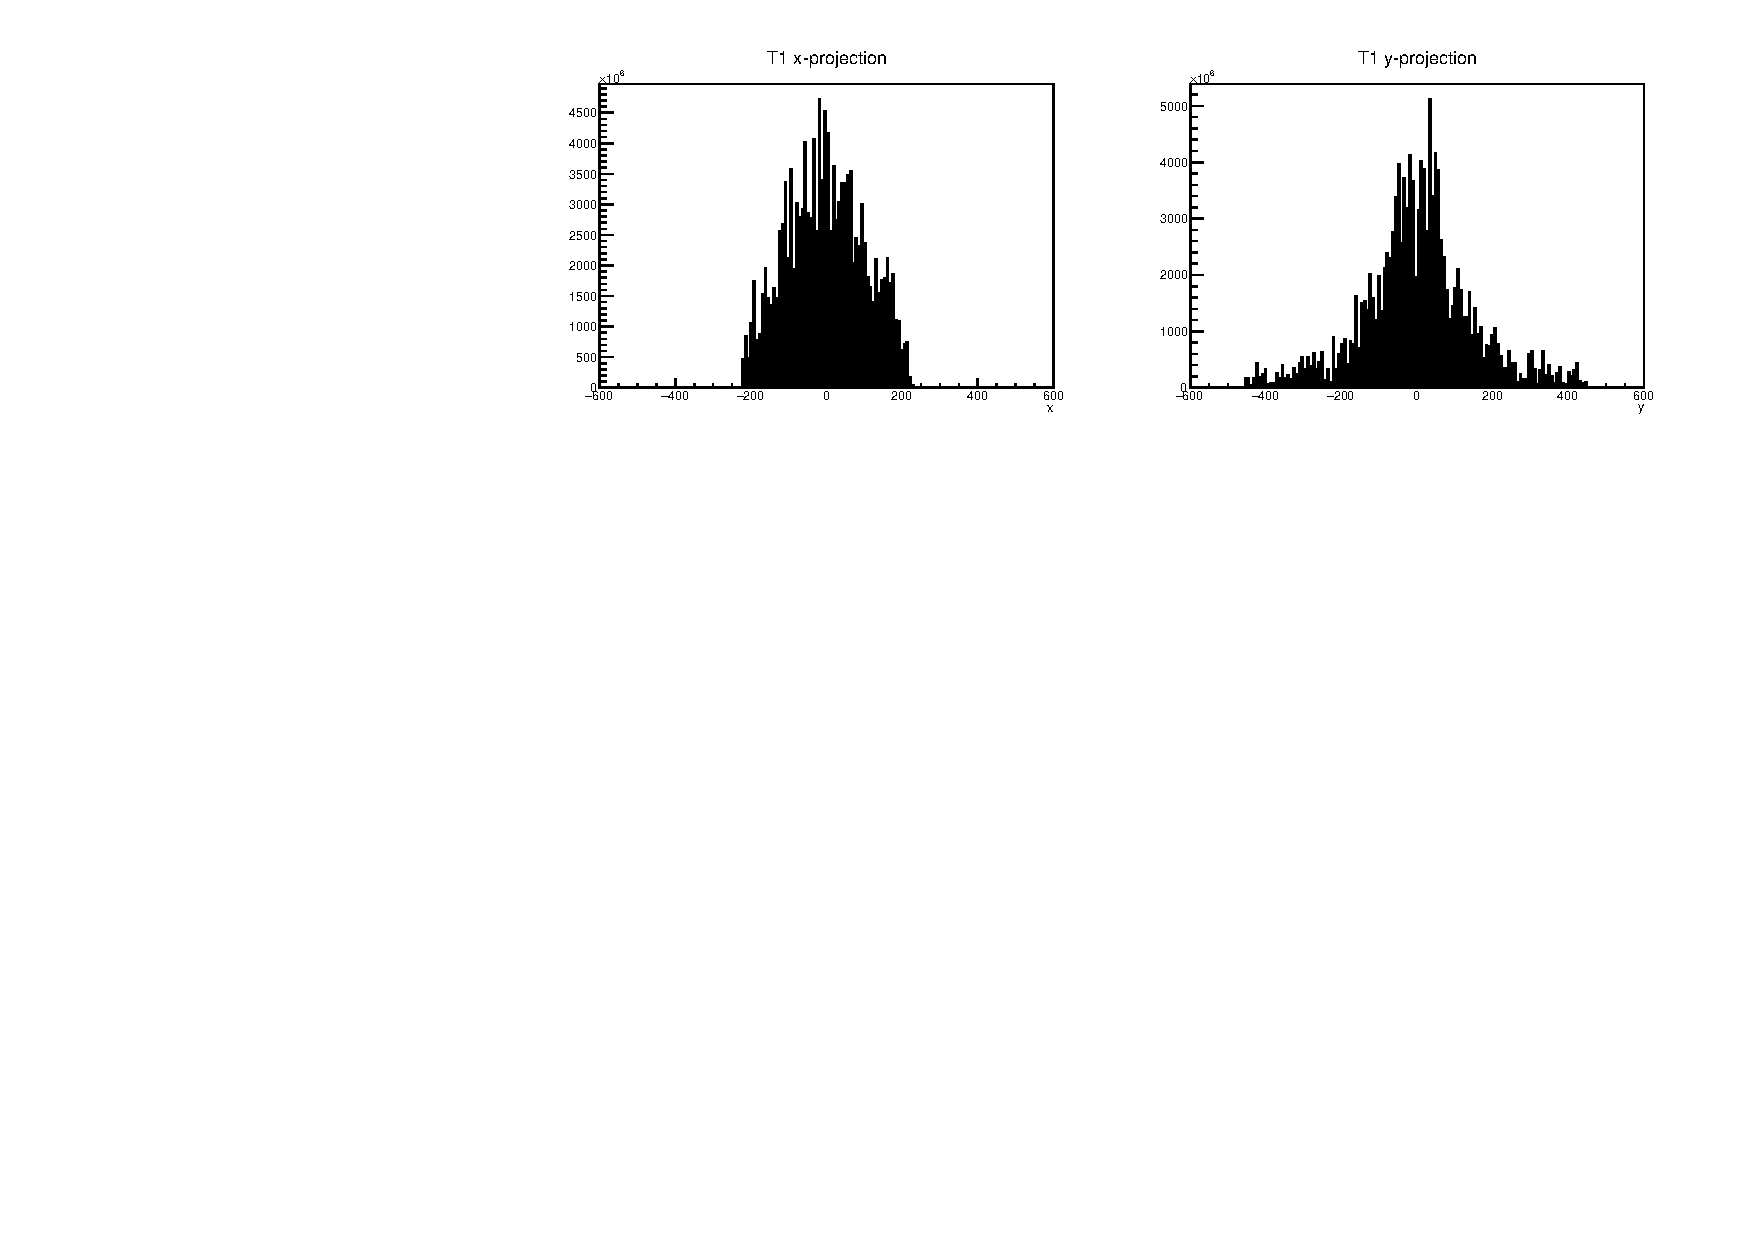
\includegraphics[width=0.9\textwidth]{../hists/strawtubes/all/proj_0.pdf}
    \end{figure}
  \vspace*{\fill}
\end{frame}

\begin{frame}[t]{}
  \begin{figure}
    \centering
    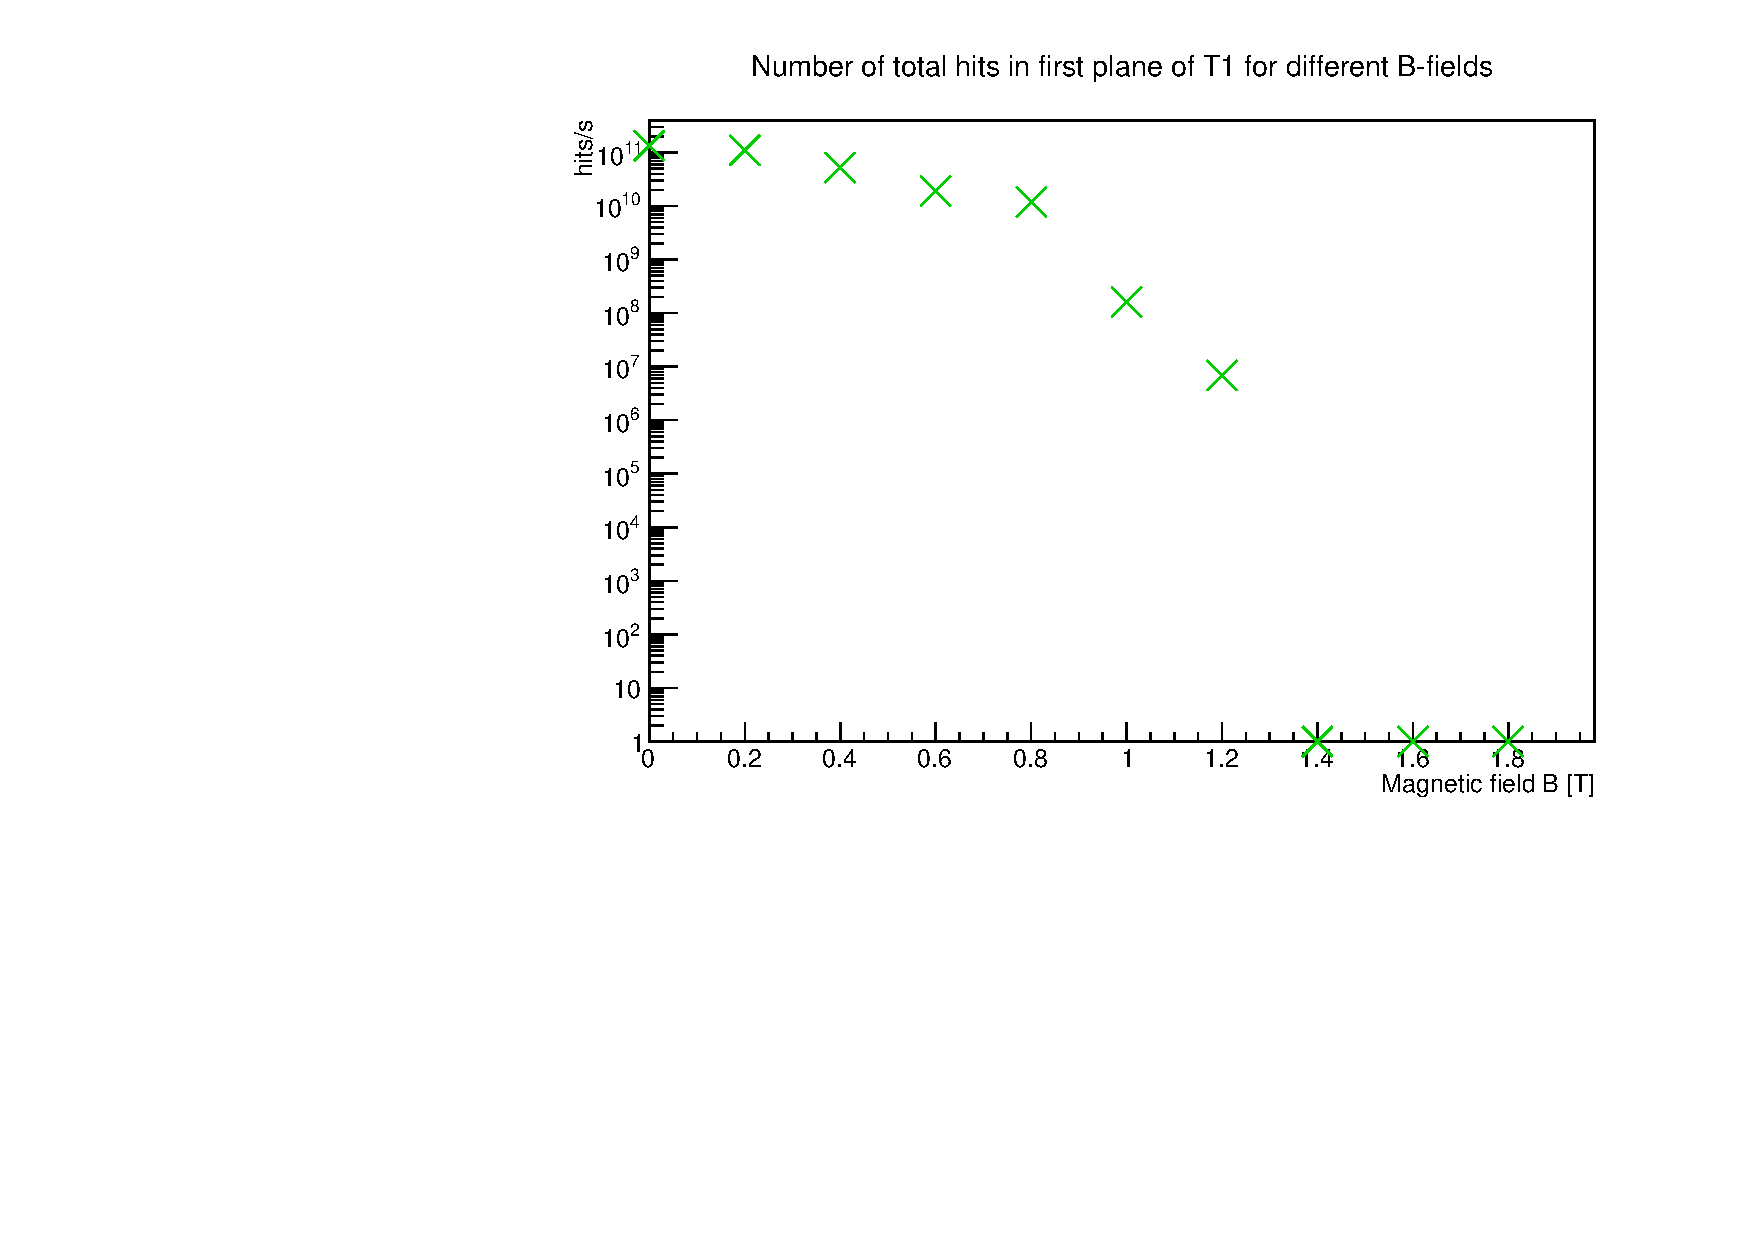
\includegraphics[width=0.78\textwidth]{../hists/strawtubes/all/hits_bfield.pdf}
  \end{figure}
\end{frame}

\begin{frame}[t]{}
  \begin{figure}
    \centering
    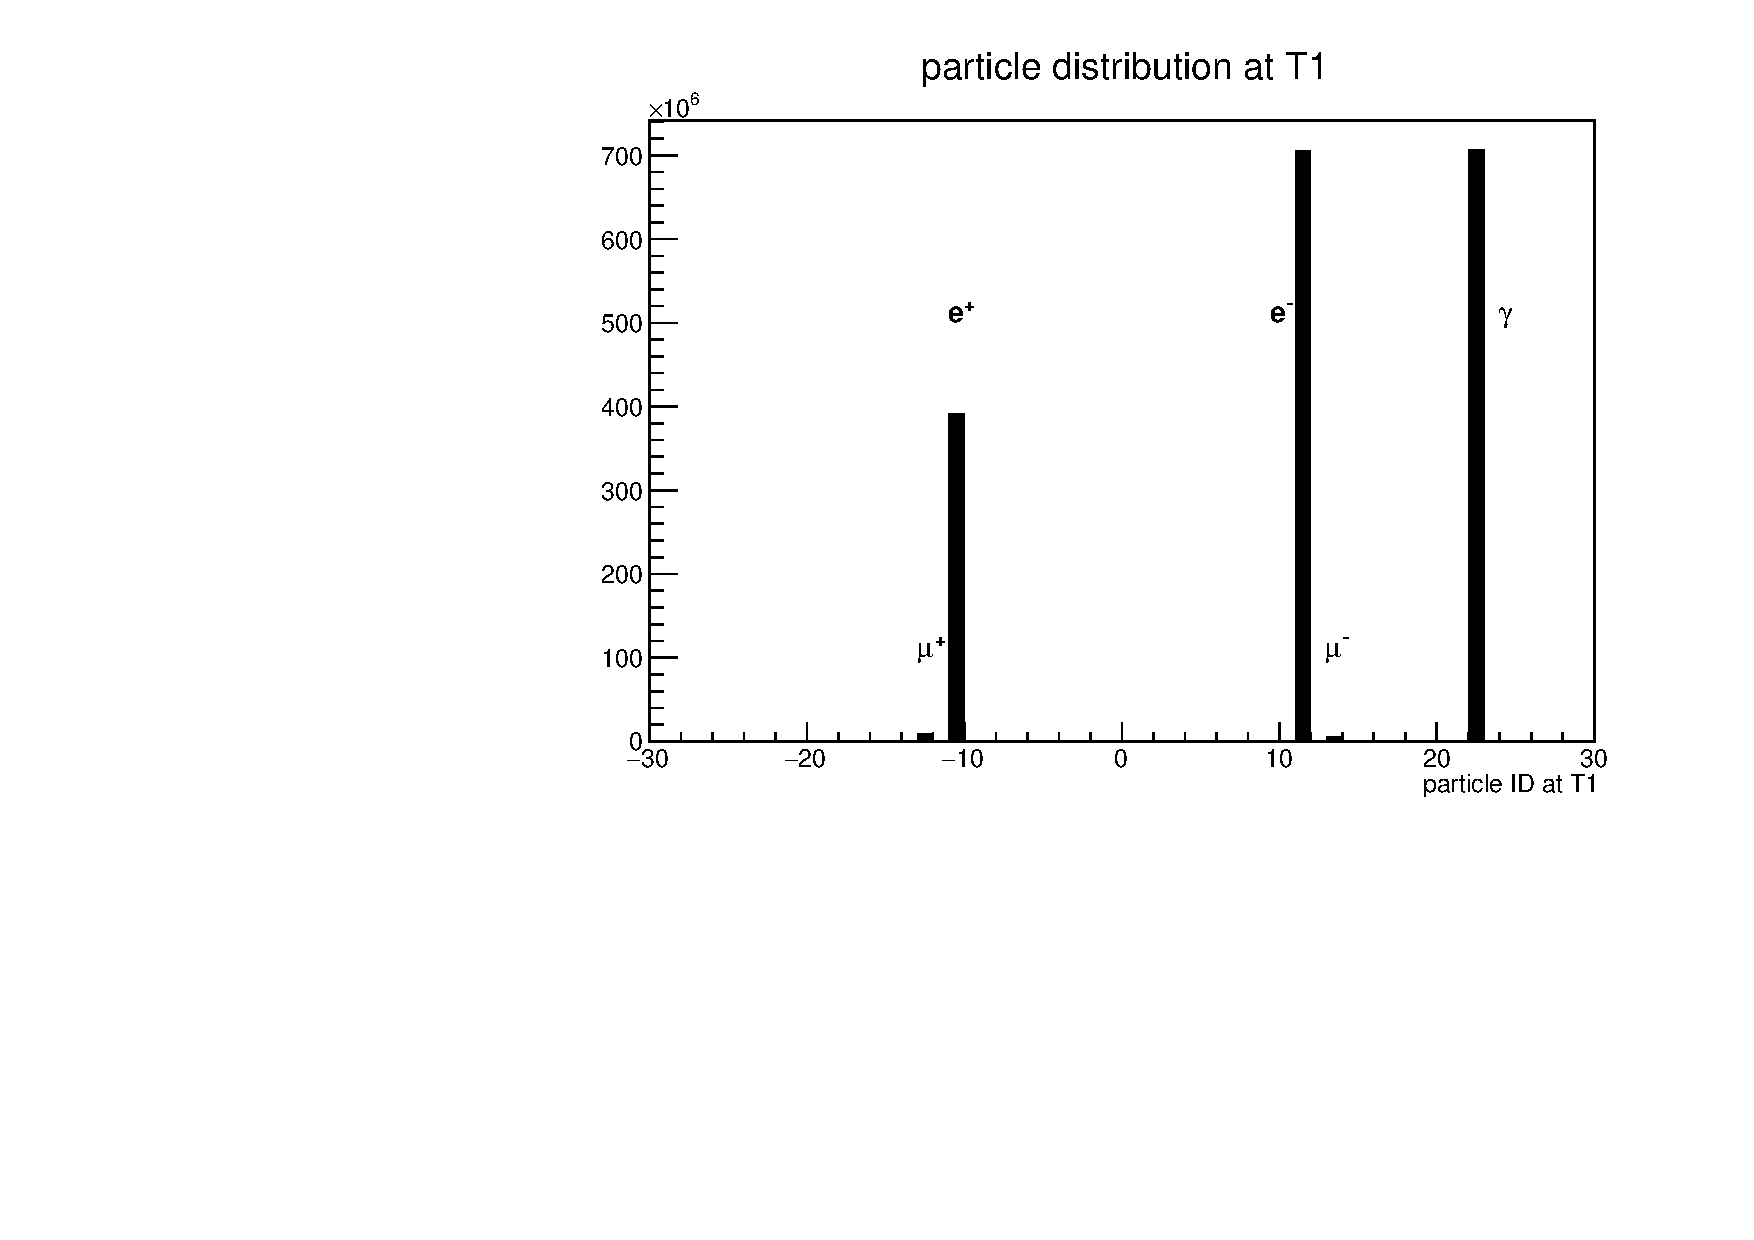
\includegraphics[width=0.65\textwidth]{../hists/strawtubes/all/pdg_T1.pdf}
  \end{figure}
\end{frame}

\begin{frame}
  \tabcolsep=0.0cm
  \begin{table}
    \centering
    \begin{tabular}{S[table-format=1.1]
                    S
                    S
                    S
                    S}
      \toprule
      {b-field [T]} & {hits/s in T1} & {hits/plane/s} & {hits/layer/s} & {hits/straw/s} \\
      \midrule
      0.0 & 1.058e12 & 1.344e11 & 6.724e10 & 1.183e8 \\
      0.2 & 8.848e11 & 1.101e11 & 5.506e10 & 9.694e7 \\
      0.4 & 4.037e11 & 5.229e10 & 2.614e10 & 4.603e7 \\
      0.6 & 1.657e11 & 1.895e10 & 9.474e9 & 1.668e7 \\
      0.8 & 8.816e10 & 1.191e10 & 5.952e9 & 1.048e7 \\
      1.0 & 7.971e8 & 1.629e8 & 8.145e7 & 1.434e5 \\
      1.2 & 2.081e7 & 6.936e6 & 3.468e6 & 6.106e3\\
      \bottomrule
    \end{tabular}
    \caption{Particle flux at T1 for different magnetic fields of the muon shield (all other fields turned off). Average calculated from hits in one plane, so the maximum rate varies locally.}
    \label{tab:mean}
  \end{table}
\end{frame}

%------------------------------------------------------------------------------------------
\section{summary}
%------------------------------------------------------------------------------------------

\begin{frame}[t]{summary}
  \vspace*{\fill}
    \begin{itemize}
      \item At first: unexpectedly large asymmetry in $x$ (no apparent physical reason)
      \item found a bug in MuonBackGenerator ($\rightarrow$ Thomas fixed it)
      \item new projection of IP looks as expected
      \item even $\SI{10}{\milli\tesla}$ remnant field in muon shield doesn't shift the mean of the distribution much ($x_{\mu^+}:\;\SI{0.50(139)}{\centi\metre}\quad\rightarrow\quad\SI{-1.16(150)}{\centi\metre}$)
      \item particle flux can be regulated by the magnetic field of the muon shield over at least 5 orders of magnitude
      \item rates at certain fields seem to be managable with tracker $\rightarrow$ further more precise studies.
    \end{itemize}
  \vspace*{\fill}
\end{frame}

%------------------------------------------------------------------------------------------
\section{outlook}
%------------------------------------------------------------------------------------------

\begin{frame}[t]{outlook}
  \vspace*{\fill}
    Of course, this can be improved. A few fields for further studies would be:
    \begin{itemize}
      \item examine bigger data samples
      \item investigate flux distribution within planes (not only average)
      \item use more exact extrapolation
      \item quantitatively compare accuracy of reconstructed IP to MC truth
    \end{itemize}
  \vspace*{\fill}
\end{frame}

%------------------------------------------------------------------------------------------
\section{Back up}
%------------------------------------------------------------------------------------------
\appendix

\begin{frame}

\end{frame}

\begin{frame}[t]{}
  \centering
  \textcolor{green}{\Huge{Back Up}}
\end{frame}



\begin{frame}[t]{Momentum distribution of the tracks}
  \begin{figure}
    \centering
    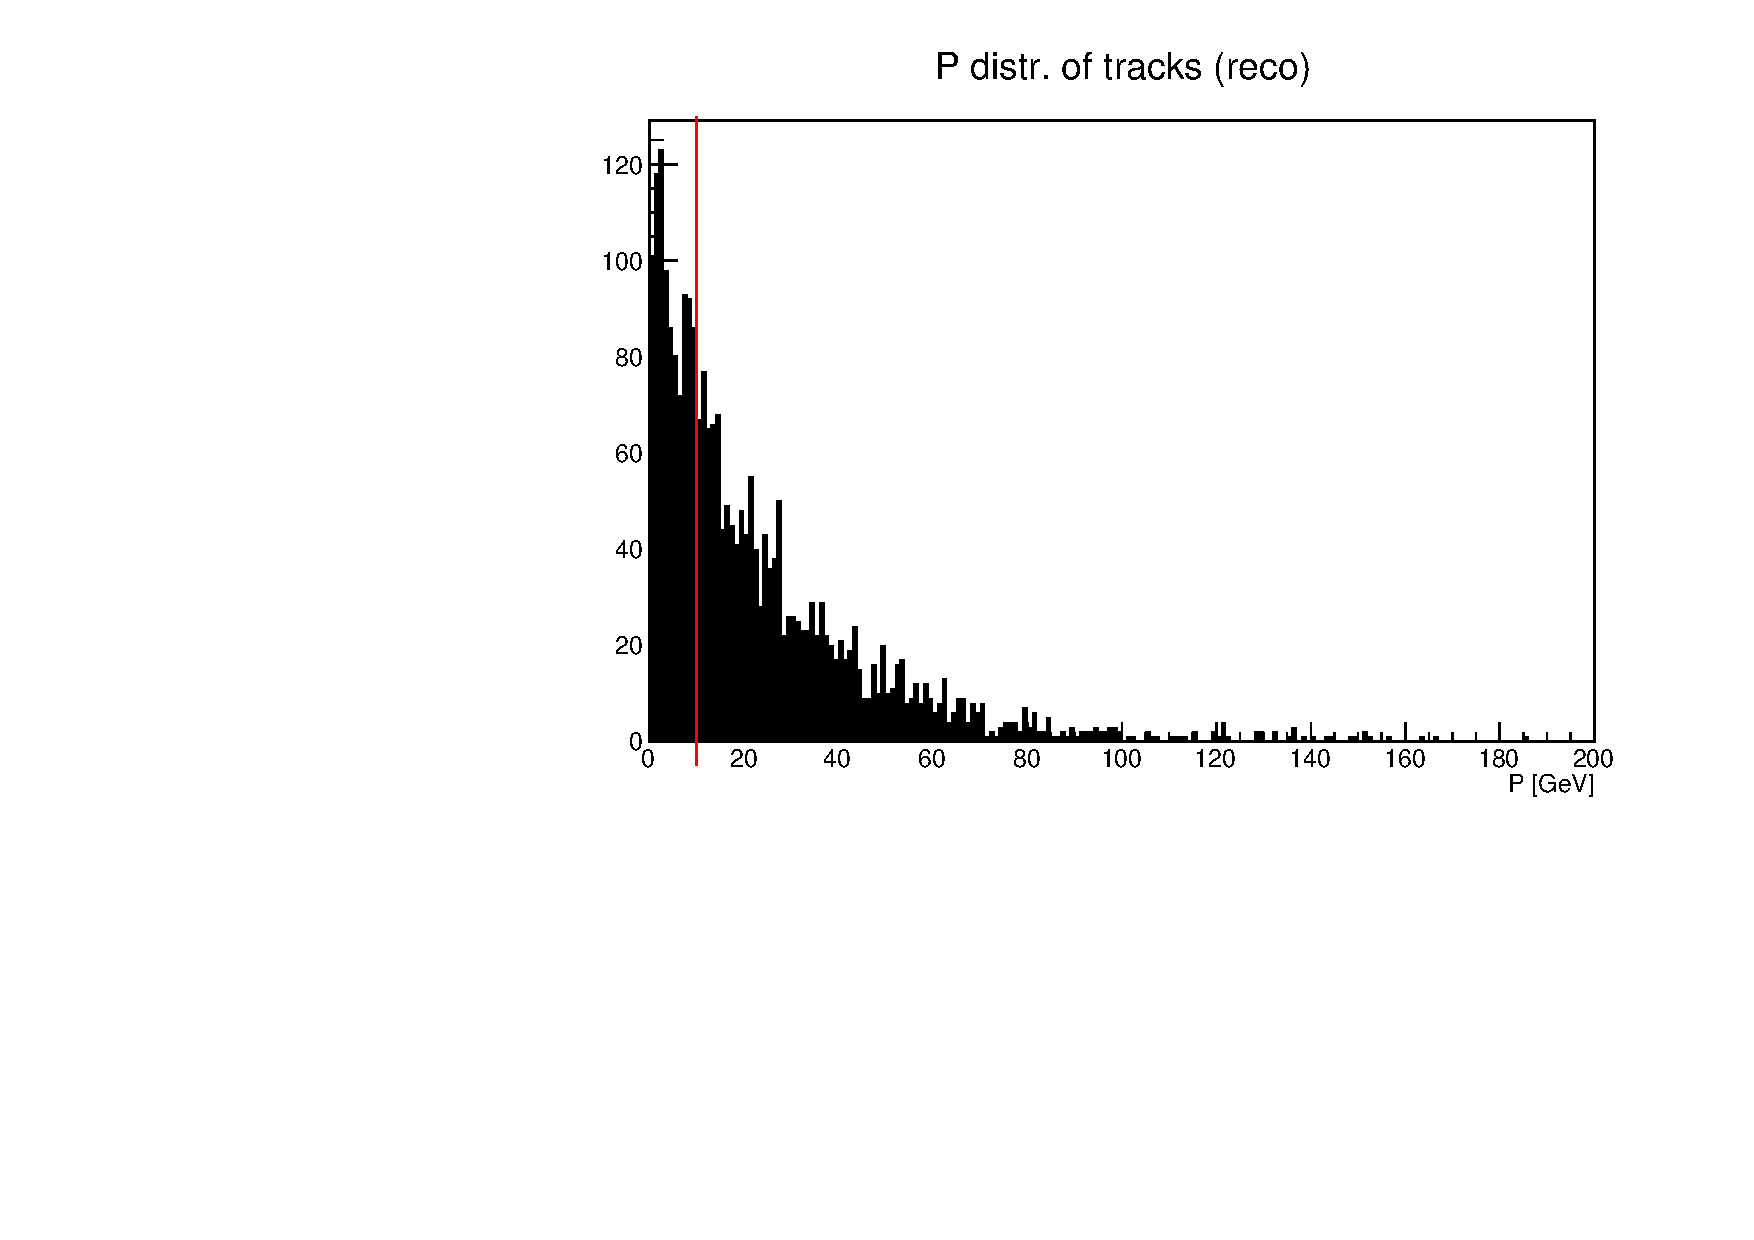
\includegraphics[width=0.65\textwidth]{../hists/nofield/mom_reco_tracks.pdf}
  \end{figure}
\end{frame}

\begin{frame}[t]{Divided for $\mu^+$ and $\mu^-$ only momenta $> \SI{10}{\giga\electronvolt}$}
  \begin{multicols}{2}
    \begin{figure}
      \centering
      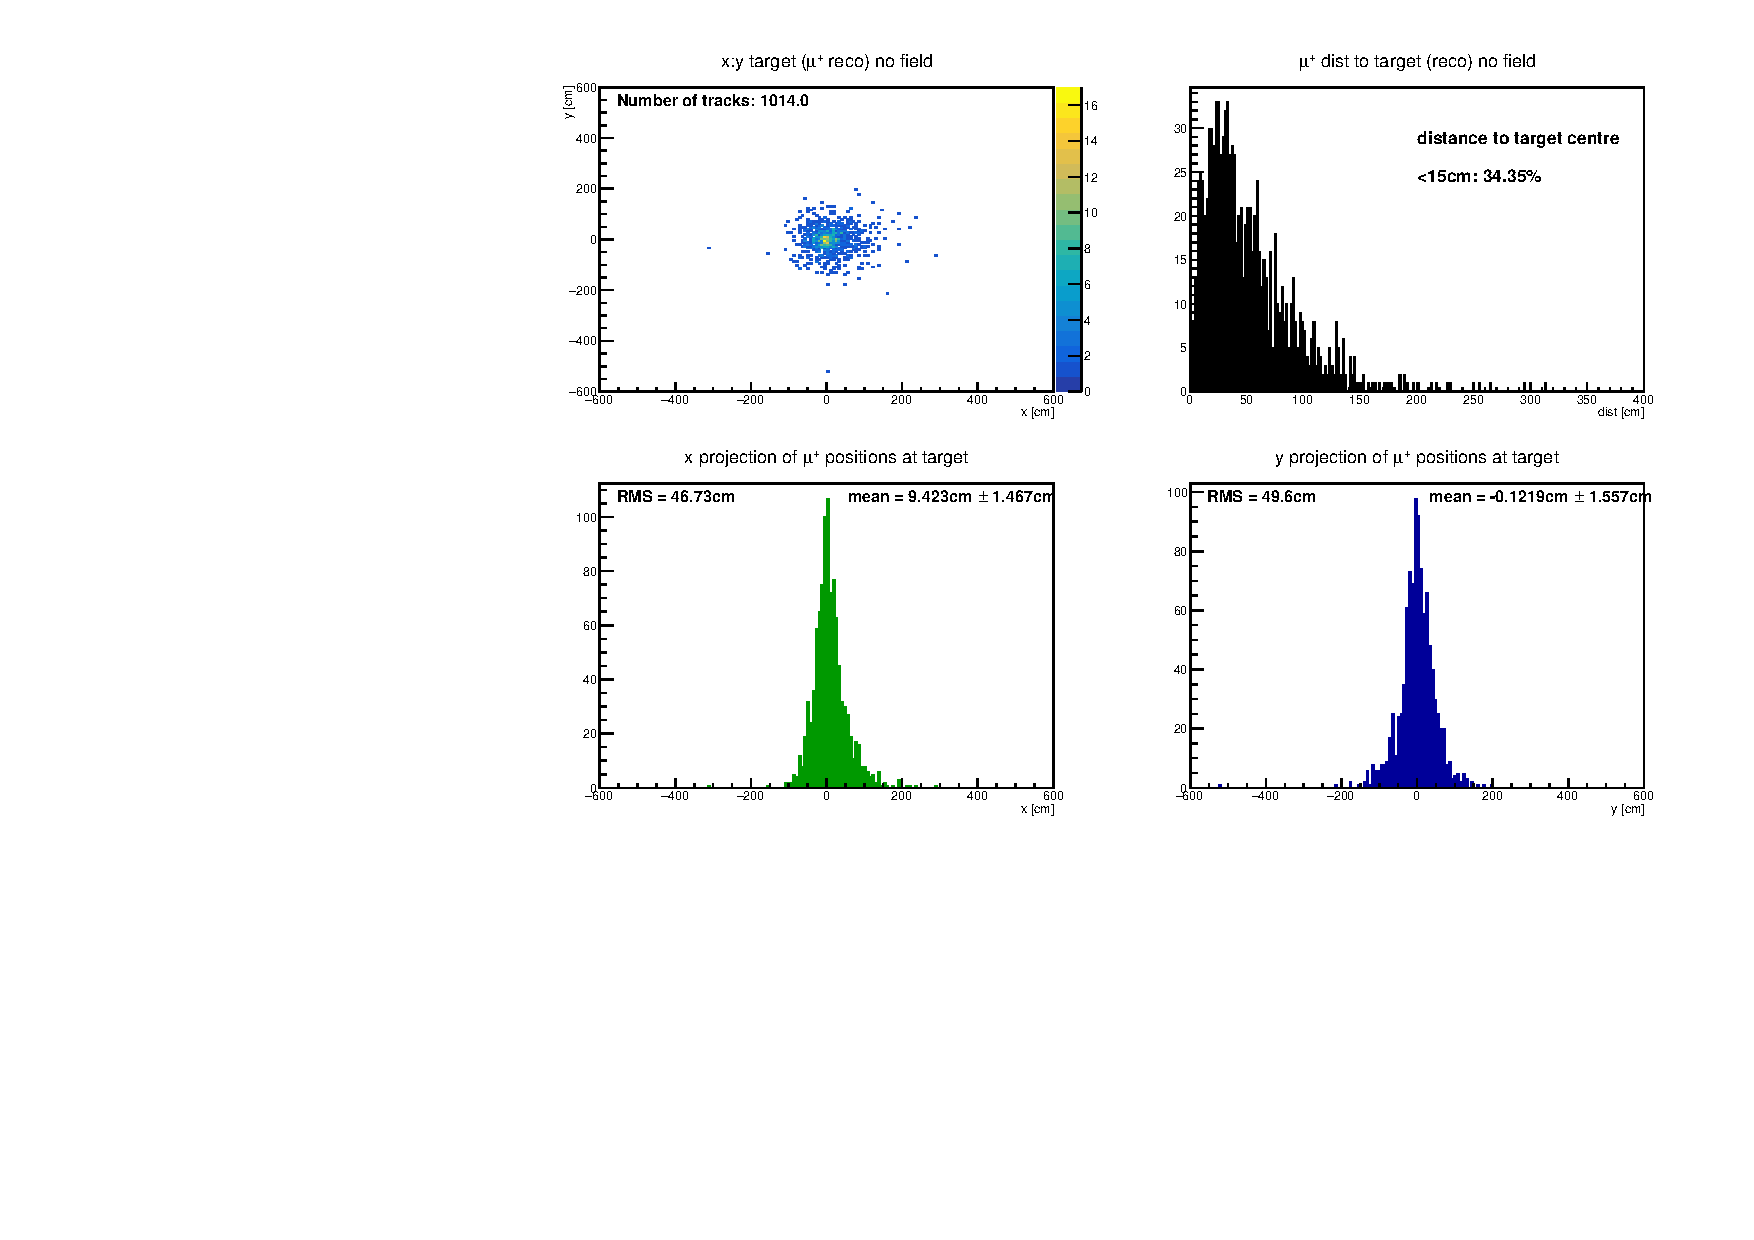
\includegraphics[width=0.5\textwidth]{../hists/nofield/P/target_dist_amu.pdf}
    \end{figure}
    \columnbreak
    \begin{figure}
      \centering
      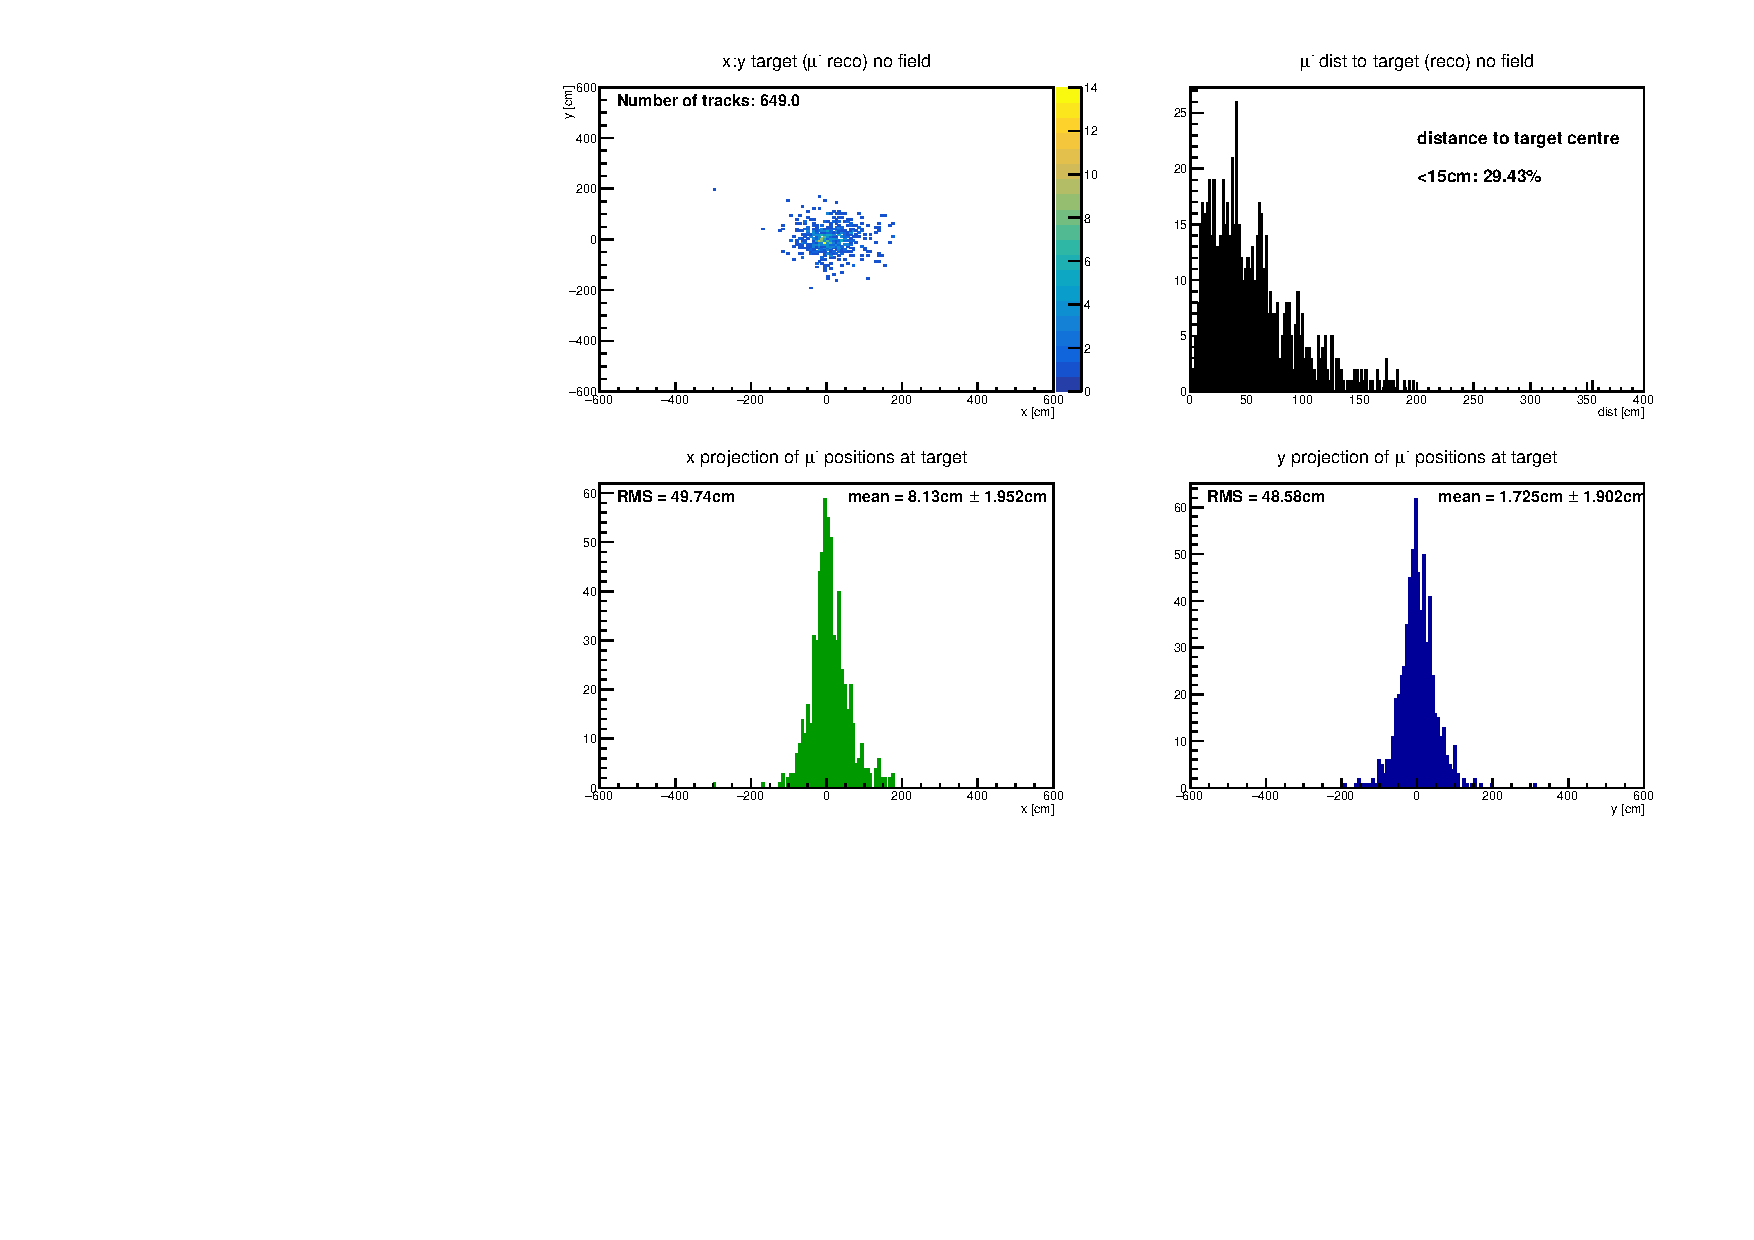
\includegraphics[width=0.5\textwidth]{../hists/nofield/P/target_dist_mu.pdf}
    \end{figure}
  \end{multicols}
\end{frame}

\begin{frame}[t]{Divided for $\mu^+$ and $\mu^-$ only momenta $< \SI{10}{\giga\electronvolt}$}
  \begin{multicols}{2}
    \begin{figure}
      \centering
      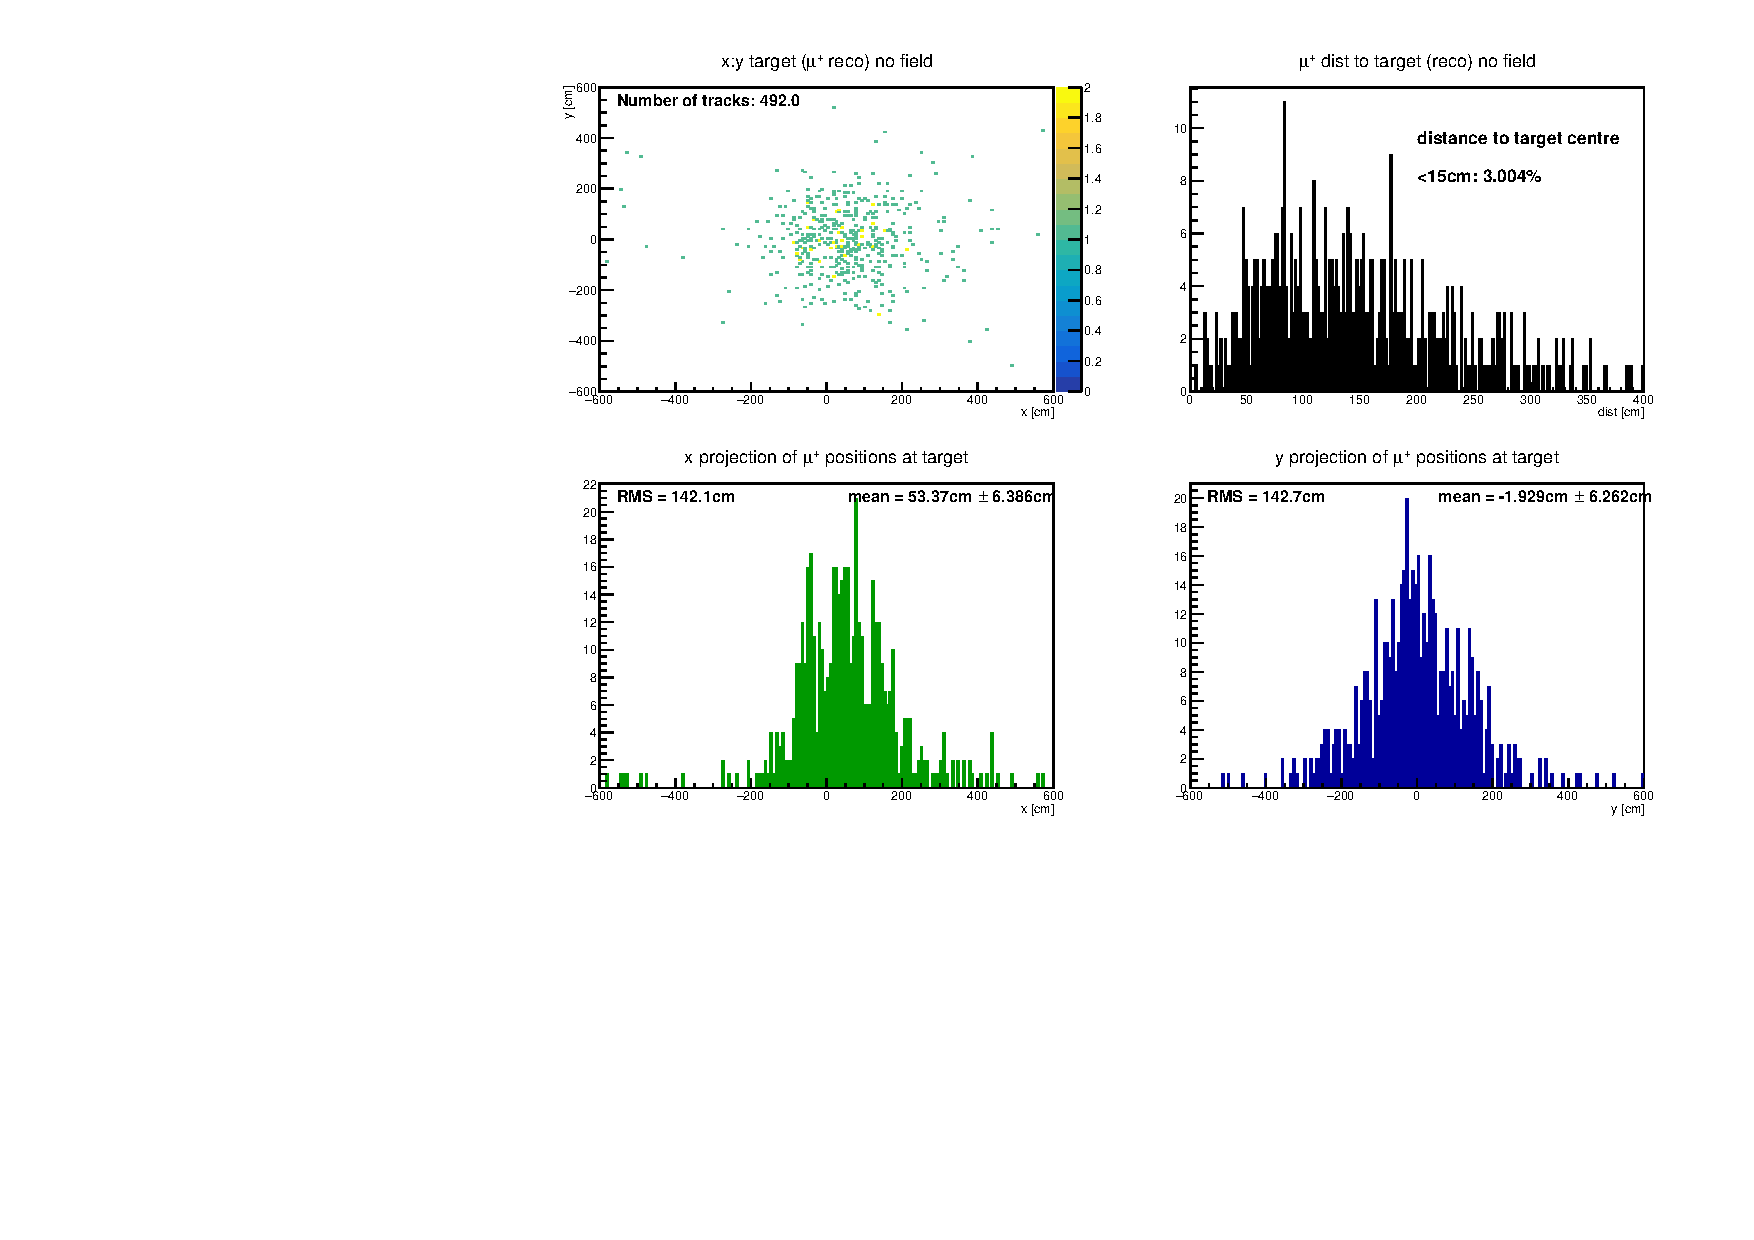
\includegraphics[width=0.5\textwidth]{../hists/nofield/p/target_dist_amu.pdf}
    \end{figure}
    \columnbreak
    \begin{figure}
      \centering
      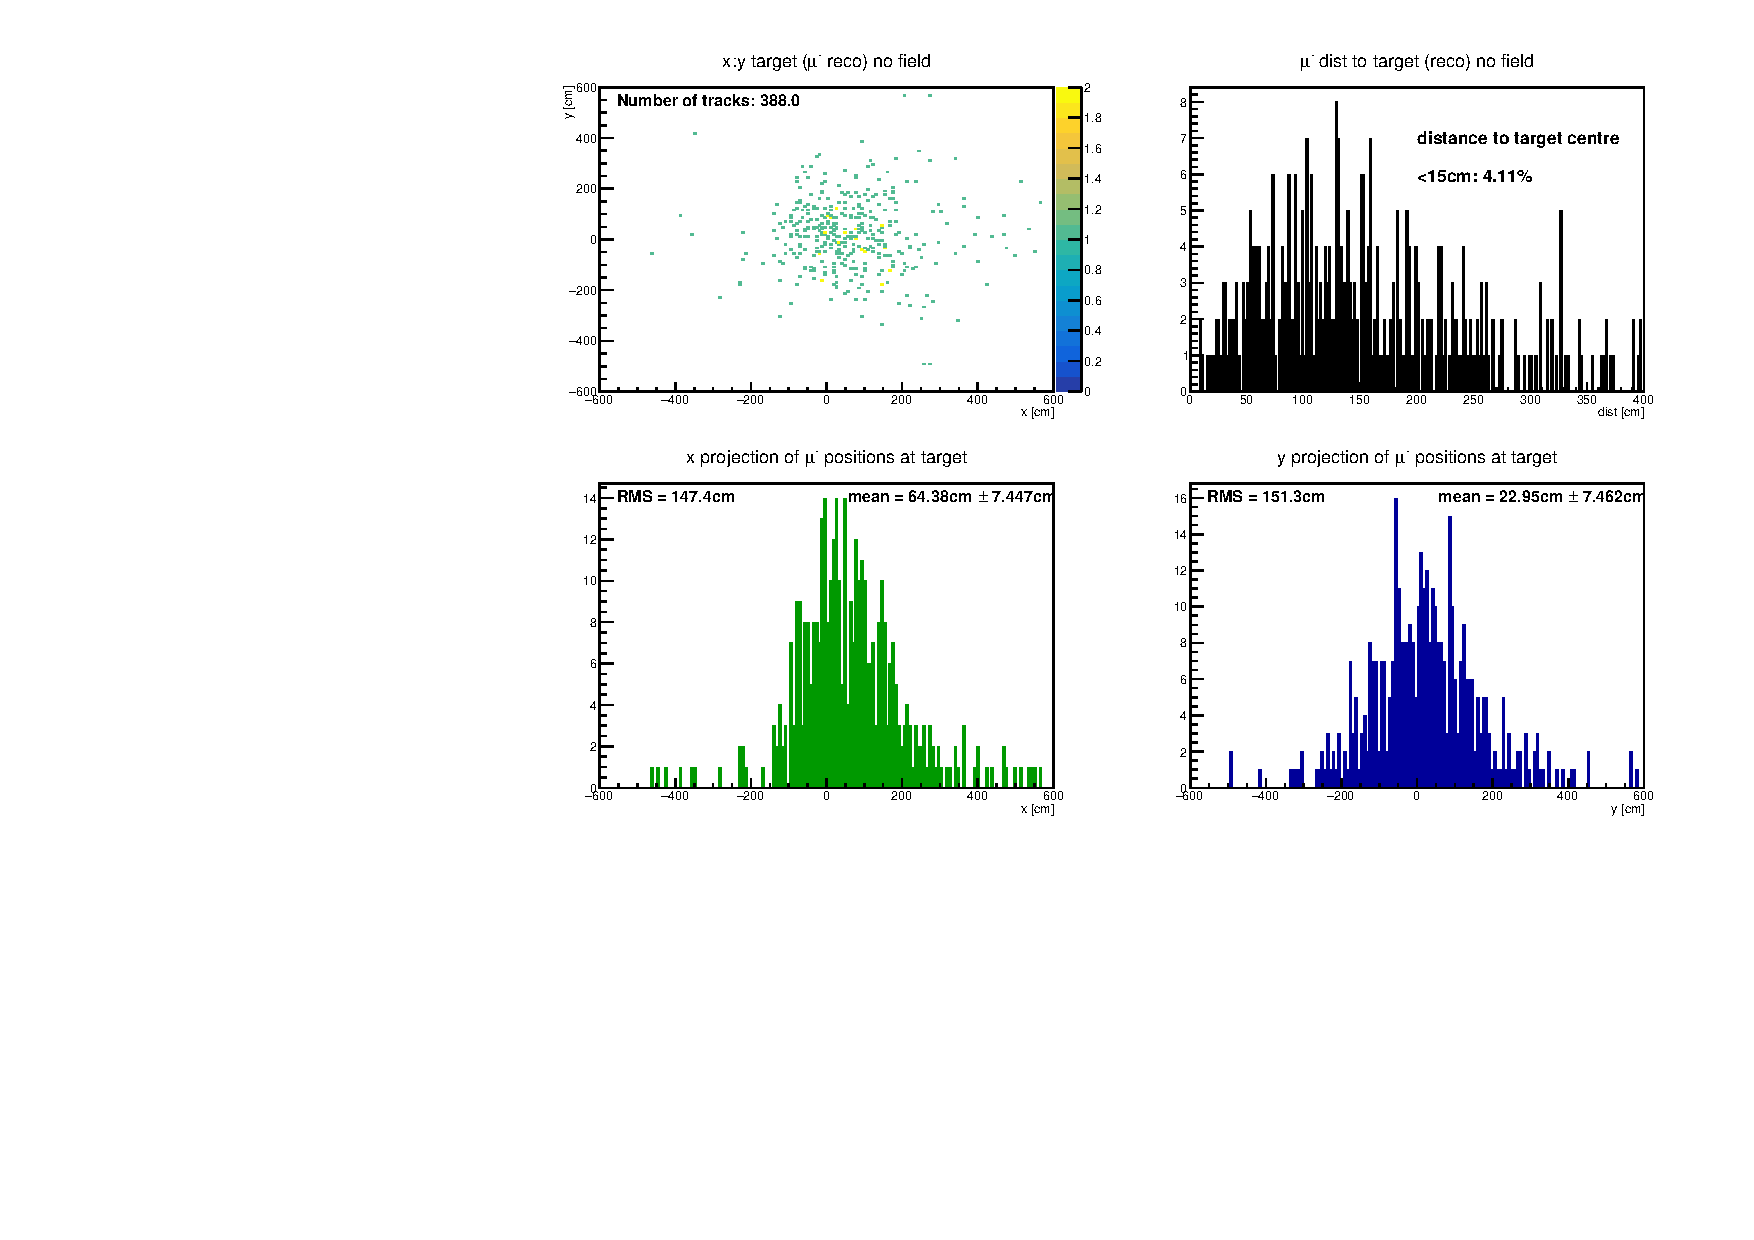
\includegraphics[width=0.5\textwidth]{../hists/nofield/p/target_dist_mu.pdf}
    \end{figure}
  \end{multicols}
\end{frame}

\end{document}
